\chapter{Literature Review}
\label{LitReview}

This chapter shall provide summaries of the background information required to understand the content of this thesis, and also review the state of the art of the various subjects that this thesis covers.

\section{Colour Science}

Organisms on earth posses visual systems such that they can glean information about spatially remote objects through the sensing of light reflected from these objects towards the organism. They are able to do this because the sun emits electromagnetic radiation (which we call `light' when it is within our visual sensitivity range), our atmosphere transmits many parts of this radiation (absorbing some wavelengths more-so than others), and objects absorb some and reflect some of this radiation (again, some wavelengths more-so than others).
%minnaert?

\begin{figure}[htbp]
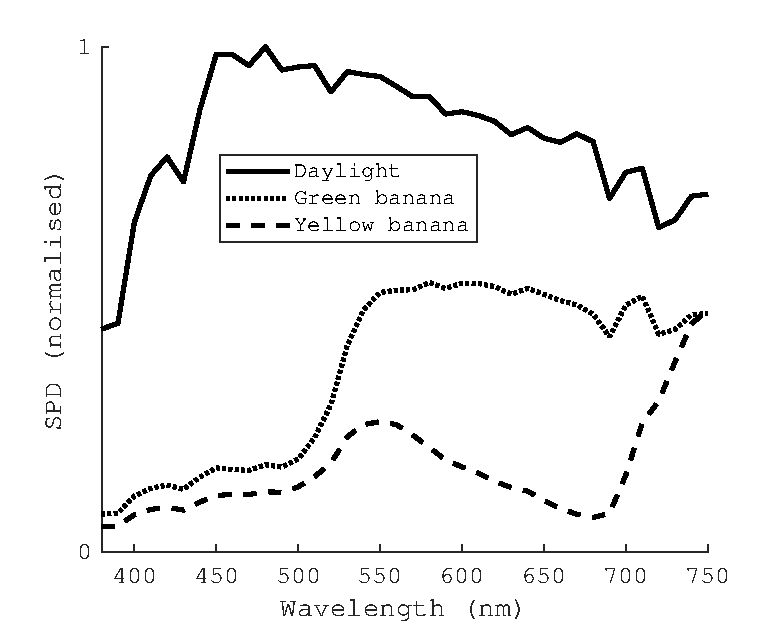
\includegraphics[max width=\textwidth]{figs/LitRev/daylightAndBananas.pdf}
\caption{The \gls{SPD} of a single measurement of daylight (sunlight plus scattered blue-sky light, from \citet{hernandez-andres_color_2001}) and the light reflected from 2 different surfaces - a green banana and a yellow banana (data from personal correspondence with David Slaughter after \citet{li_optical_1997}), computed by multiplying the \gls{SPD} by the measured \glspl{SRF} of the two surfaces. \Glspl{SPD} normalised such that the max of the daylight \gls{SPD} is 1.}
\label{fig:SPD}
\end{figure}

Our perception of colour generally correlates with the way in which objects preferentially reflect some wavelengths over others (described by the \acrfull{SRF}) which assists in the recognition of objects (that's a banana) and the discrimination of distinct objects, often in a manner that it ecologically beneficial (that's a \emph{ripe} banana).

\subsection{Colorimetry}

\textit{The current recommended source for colorimetry is \gls{CIE} document `\gls{CIE} 015:2018'\citep{cie_cie_2018}\footnote{Though as \citet{fairchild_cie_2019} notes, this document is `expensive and somewhat difficult to find', and as such I have been using a draft of the now superseded `\gls{CIE} 15.3:2004'\citep{cie_cie_2004-2} as my personal guide. All equations listed in this chapter come from this source.}. Whilst this is the authoritative reference, my personal opinion is that an understanding of \gls{CIE} colorimetry is best gained from an understanding of its history, and for this I recommend Janos Schanda's book `Colorimetry: Understanding the \gls{CIE} System' \citep{schanda_colorimetry_2007}. Another valuable, and perhaps more easily accessed, reference source is \citet{stockman_color_2010}.}

\bigskip

I define `colorimetry' as the study of the quantitative specification of colour. As a subjective, internal and anthropocentric concept, in order to measure anything meaningful and comparable, we use a standard observer, or more precisely, one of a number of defined standard observers \cite{cie_bs_2011}.

The classic standard observer was defined by the \gls{CIE} in 1931, following experiments by Wright and Guild \cite{wright_re-determination_1929, guild_colorimetric_1931}. Despite several more recently published standard observers, the 1931 observer is still much used, and I shall use it in the following example of how a basic colorimetric computation is performed.

\glsreset{SPD}
\glsreset{SRF}
\glsreset{CMF}
\glsreset{SSF}

An illuminant is defined by its \gls{SPD}, a surface by its \gls{SRF}, and the sensitivity of a sensor (such as a photosensitive cell in the retina, or a pixel in a camera) by its \gls{CMF} (or in the case that biologically based measurements are used - the \gls{SSF}).

\begin{figure}[htbp]
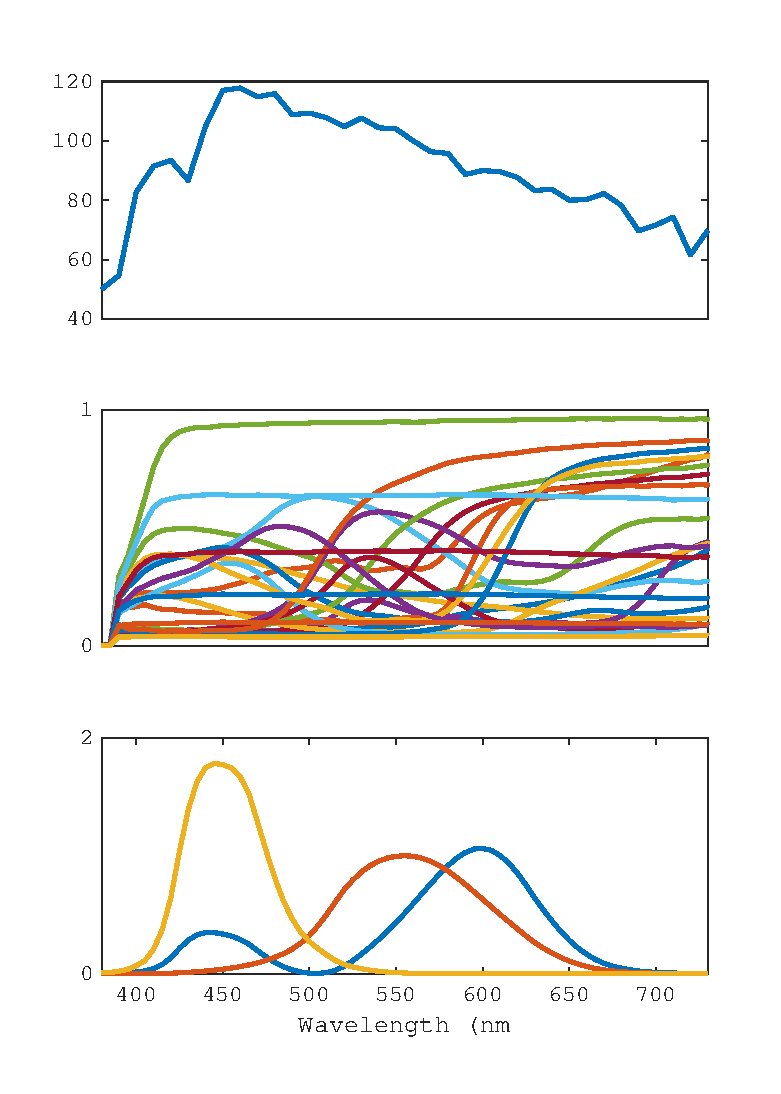
\includegraphics[max width=\textwidth]{figs/LitRev/SPDetc.pdf}
\caption{An \gls{SPD} (D65), a set of \glspl{SRF} (from a Macbeth Colour Checker) and three \glspl{CMF} (\gls{CIE} 1931 observer).}
\label{fig:specFun}
\end{figure}
% % How is D65 normalised here?

The light reaching the eye for a given reflecting surface under a given illuminant (termed the `colour signal') can be computed by multiplying the \gls{SPD} by the \gls{SRF} at each sampled interval.

\begin{equation}
\phi(\lambda)=R(\lambda) \cdot S(\lambda)
\end{equation}

where $R(\lambda)$ is the \gls{SRF}, $S(\lambda)$ is the \gls{SPD} and $\phi(\lambda)$ is the resulting colour signal. From this a set of values termed `tristimulus values' may be computed. Tristimulus values are computed by multiplying the colour signal by the \glspl{CMF} or \glspl{SSF}, and following the principle of univariance (that each cone type cannot alone distinguish between different wavelengths) the tristimulus values can, to some extent, be thought of as containing the entirety of the chromatic information about a surface (for a human standard observer, excluding high level colour appearance phenomena predicted by \Glspl{CAM}, and properties such as gloss).

%KC: make sure these equations are on the same page as the explanation 

\begin{subequations}
\begin{align}
X=k \sum_{\lambda} \phi(\lambda) \overline{x}(\lambda) \Delta \lambda \\ 
Y=k \sum_{\lambda} \phi(\lambda) \overline{y}(\lambda) \Delta \lambda \\ 
Z=k \sum_{\lambda} \phi(\lambda) \overline{z}(\lambda) \Delta \lambda
\end{align}
\label{eq:XYZ}
\end{subequations}

\nopagebreak %this doesn't work currently

where $\overline{x}(\lambda)$ (said `x bar'), $\overline{y}(\lambda)$ and $\overline{z}(\lambda)$ are the \glspl{CMF} of the 1931 observer (or are replaced by the \Glspl{CMF}/\Glspl{SSF} of the chosen observer), $\phi(\lambda)$ is as defined above, $k$ is a normalising factor, and $\Delta\lambda$ is 1nm. It is traditional to set $k$ such that $Y=100$, though in the case of relative colorimetry (most cases) this is often not done since the following equation renders it superfluous.

From the tristimulus values ($X,Y$ and $Z$) chromaticity co-ordinates ($x$ and $y$) can be computed. These can then be plotted on a 1931 chromaticity space diagram, shown as Figure \ref{fig:1931}.

\begin{subequations}
\begin{align}
x=\frac{X}{X+Y+Z} \\
y=\frac{Y}{X+Y+Z} 
\end{align}
\label{eq:1931chrom}
\end{subequations}

% Here's a \gls{MATLAB} example, using \gls{PTB} for data:

% \begin{lstlisting}[language=MATLAB]
% load spd_D65 % SPD: CIE D-series illuminant D65
% load sur_macbeth % SRF: macbeth colour checker
% load T_xyz1931 % CMF: CIE 1931

% colourSignals = sur_macbeth.*spd_D65;
% XYZ = T_xyz1931*colourSignals;
% xy = [XYZ(1,:)./sum(XYZ);XYZ(2,:)./sum(XYZ)];
% \end{lstlisting}

% Plotting: 

% \begin{lstlisting}[language=MATLAB]
% spectralLocus = [T_xyz1931(1,:)./sum(T_xyz1931);T_xyz1931(2,:)./sum(T_xyz1931)];
% sRGBSpectralLocus = XYZToSRGBPrimary(T_xyz1931);

% figure, hold on, 
% scatter(spectralLocus(1,1:70),spectralLocus(2,1:70),[],sRGBSpectralLocus(:,1:70)','filled')
% scatter(xy(1,:),xy(2,:),'k')
% axis equal, axis([0 1 0 1])
% xticks([0 1]), yticks([0 1])
% xlabel('x'), ylabel('y')
% \end{lstlisting}

\begin{figure}[htbp]
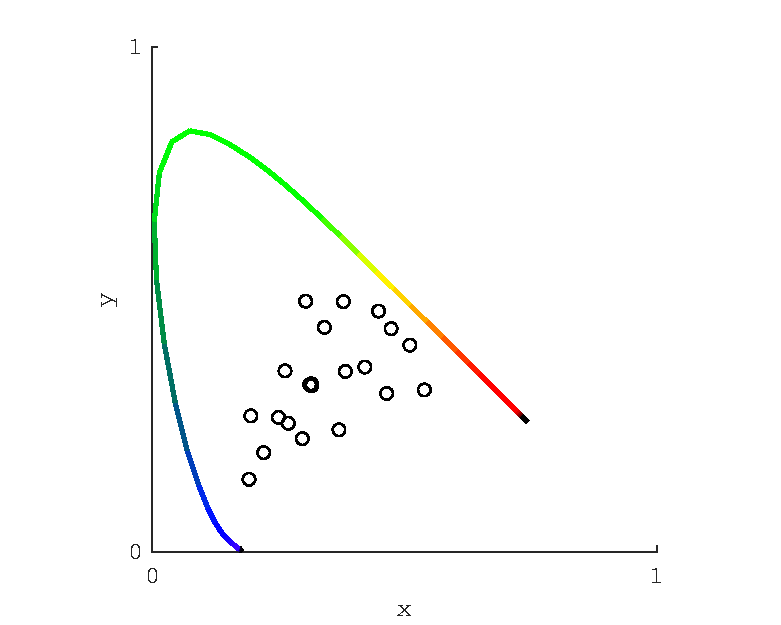
\includegraphics[max width=\textwidth]{figs/LitRev/ColorimetryDemo1.pdf}
\caption{The \gls{CIE} 1931 chromaticity space, showing the chromaticity of the Macbeth colour checker patches under D65. Note that for all of the plots in this section, the colours used for the spectral loci are only approximations.}
\label{fig:1931}
\end{figure}

\subsubsection{Specific Colour Spaces} \label{sec:speccolspac}

Over time various other colour spaces have been proposed and formally accepted by the \gls{CIE}, each aiming to improve upon a prior space in one or more ways. One of the most frequently sought characteristics for a colour space is perceptual uniformity, whereby a set distance in one part of the space is comparable in terms of apparent colour difference to that same distance in another part of the space.

One such chromaticity space which shall be used extensively in this thesis is the \gls{CIE} 1976 UCS (uniform chromaticity scale) space (colloquially \gls{CIE} u'v'), which is a relatively simple transformation of the 1931 chromaticity space. The conversion can be accomplished in a number of analogous fashions, one of which is shown below.

\begin{subequations}
\begin{align}
u' &= 4x / (-2x + 12y + 3) \\
v' &= 9y / (-2x + 12y + 3)
\end{align}
\end{subequations}

where $x$ and $y$ are the 1931 chromaticity co-ordinates as defined in Equation \ref{eq:1931chrom}. The data presented in Figure \ref{fig:1931} are re-plotted in this new space in Figure \ref{fig:UCS}.

\begin{figure}[htbp]
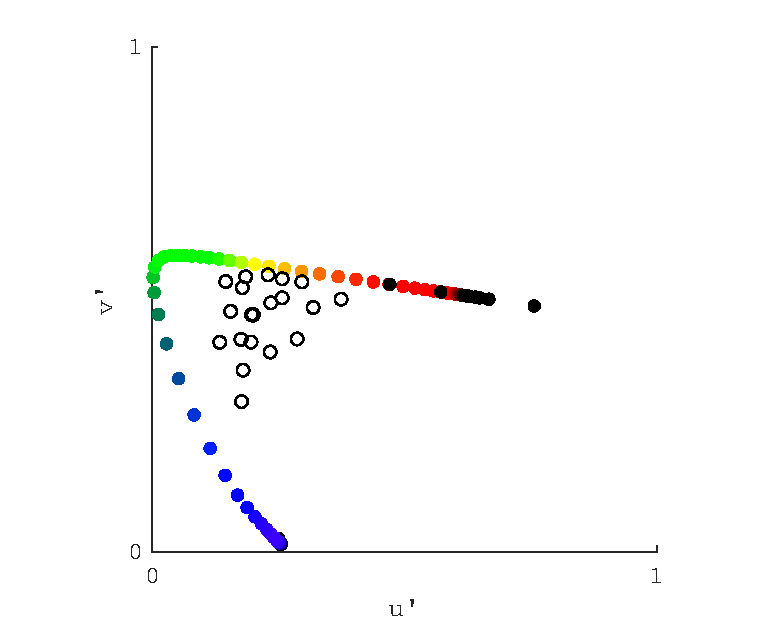
\includegraphics[max width=\textwidth]{figs/LitRev/ColorimetryDemo3.pdf}
\caption{\gls{CIE} 1976 UCS (uniform chromaticity scale) space, showing the chromaticity of the macbeth colour checker patches under D65 (as in Figure \ref{fig:1931}).}
\label{fig:UCS}
\end{figure}

A three-dimensional extension to the CIE 1976 UCS space is the \gls{CIE} 1976 L*u*v* colour space, often abbreviated to CIELUV, which aims to provide perceptual uniformity in a space that includes both chromaticity and lightness (relative to a white object under the same illumination). It is defined as follows:

\begin{subequations}
\begin{align}
L^{*} &= 116 f(Y/Y_{n})-16 \\
\textrm{where} f(Y/Y_{n}) &= (Y/Y_{n})^{1/3} &\textrm{ if } (Y/Y_{n}) > (24/116)^{3} \\
\textrm{or} f(Y/Y_{n}) &= (841/108)(Y/Y_{n})+16/116 &\textrm{ if } (Y/Y_{n}) \leq (24/116)^{3} \\
u^{*} &= 13L^{*}(u'-u'_{n}) \\ 
v^{*} &= 13L^{*}(v'-v'_{n})
\end{align}
\end{subequations}

where $Y_{n}$, $u'_{n}$ and $v'_{n}$ refer to the colour stimulus of a perfect reflector. The same data presented in Figures \ref{fig:1931} and \ref{fig:UCS} is presented in CIELUV in Figure \ref{fig:CIELUV} (though of course the three-dimensional quality of the data is somewhat lost in this presentation). 

\begin{figure}[hbtp]
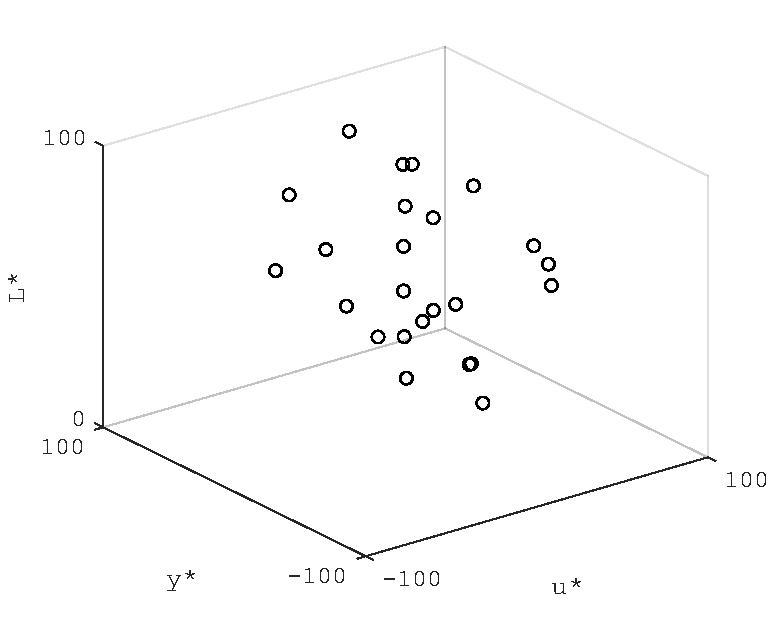
\includegraphics[max width=0.8\textwidth]{figs/LitRev/ColorimetryDemo4.pdf}
\caption{A representation of CIELUV, showing the values for the macbeth colour checker patches under D65 (as in Figure \ref{fig:1931} and \ref{fig:UCS}). Note that if viewed from above, the distribution of points would appear similar to as in Figure \ref{fig:UCS}. If all of the points were of uniform $L^{*}$, then the distribution would be identical, only with different scaling and offsetting.}
\label{fig:CIELUV}
\end{figure}

Introduced at the same time as CIELUV was a colourspace with a similar goal of perceptual uniformity: CIELAB. They are similar in many ways, and share $L^{*}$. CIELAB seems to be in slightly more common usage, but CIELUV is used in this thesis (particularly Chapter \ref{chap:Tablet}) due to the neat mathematical link to an associated chromaticity space (the CIE 1976 UCS space). 

The two spaces suit subtly different purposes, requested by two different user groups identified at the time of the creation of these spaces: ``lighting engineers interested in a space and formula that is a linear transformation of the CIE chromaticity diagram, and industrial colorists interested in a formula predicting perceived average color differences better than any existing one'' \citep{kuehni_color_2008}. CIELUV satisfied the first group, and CIELAB was designed to better suit the second, using a cube root function for the chromaticity values, mirroring $L^{*}$. CIELAB is defined as follows:

\begin{subequations}
\begin{align}
L^{*} &= 116 f(Y/Y_{n})-16 \\
\textrm{where} f(Y/Y_{n}) &= (Y/Y_{n})^{1/3} &\textrm{ if } (Y/Y_{n}) > (24/116)^{3} \\
\textrm{or} f(Y/Y_{n}) &= (841/108)(Y/Y_{n})+16/116 &\textrm{ if } (Y/Y_{n}) \leq (24/116)^{3} \\
a^{*} &= 500[f(X/X_{n}) - f(Y/Y_{n})] \\ 
b^{*} &= 200[f(Y/Y_{n}) - f(Z/Z_{n})] 
\end{align}
\end{subequations}

where $f(X/X_{n})$ and $f(Z/Z_{n})$ follow the same format as $f(Y/Y_{n})$.

The final colour space presented here is the \acrfull{MB} colour space. This space does not aspire to be perceptually uniform\footnote{This can be clearly noted by comparing Figure \ref{fig:lrMB} with previous figures. Where this set of chromaticities previously spanned the spaces fairly broadly, here all the chromaticities inhabit only a small portion of the chromaticity space.}. Instead, it aspires to provide a colour space which has a physiological underpinning. As such, the standard observer model consists of nominal \glspl{SSF} (rather than \glspl{CMF}), and the conversion from tristimulus values to chromaticity space attempts to mirror the way in which this actually occurs physiologically.

It was originally proposed by \citet{macleod_chromaticity_1979}, but was recently revised and endorsed by the \gls{CIE}, in documents `CIE 170-1:2006' \citep{cie_cie_2006} and `CIE 170-2:2015' \citep{cie_cie_2015}\footnote{I understand that the final publication in the series (`CIE 170-3:XXXX') is in preparation.}. The revisions included the definition of a new observer (formally the `TC 1-36 Modified Colorimetric Observer', colloquially refered to as the \gls{CIE} 2006 observer), based on the work of \citet{stockman_spectral_1999} and \citet{stockman_spectral_2000} (and referred to below as $\overline{lms}$), and the introduction of a set of new normalising terms, such that it is now calculated as follows.

\begin{subequations}
\begin{align}
L_{\text{MB}}&=k_{l} \sum_{\lambda} \phi(\lambda) \overline{l}(\lambda) \Delta \lambda \\ 
M_{\text{MB}}&=k_{m} \sum_{\lambda} \phi(\lambda) \overline{m}(\lambda) \Delta \lambda \\ 
S_{\text{MB}}&=k_{s} \sum_{\lambda} \phi(\lambda) \overline{s}(\lambda) \Delta \lambda
\end{align}
\label{eq:MBTristim}
\end{subequations}

where $k_{l}$ = 0.68990272, $k_{m}$ = 0.34832189, $k_{s}$ = 0.03715971. This set differs minimally but purposefully from Equation \ref{eq:XYZ}; in the choice of observer ($\overline{lms}$), and in the use of different scaling factors for each tristimulus value. The different scaling values dictate the relative contributions of $L_{\text{MB}}$ and $M_{\text{MB}}$ to luminance, and constrict $s_{\text{MB}}$ to a maximum value of 1 in the following equation (Equation \ref{eq:MB}). \gls{MB} chromaticity values are then calculated as follows:

\begin{subequations}
\begin{align}
l_{\text{MB}}&= \frac{L_{\text{MB}}}{L_{\text{MB}}+M_{\text{MB}}} \\ 
s_{\text{MB}}&= \frac{S_{\text{MB}}}{L_{\text{MB}}+M_{\text{MB}}} 
\end{align}
\label{eq:MB}
\end{subequations}

Whereas the relationship between the axes of previous colour spaces was important, here the axes are nominally independent (representing different post-receptoral mechanisms) and so the scaling between the axes is arbitrary. As such, in vision science the axes of this diagram are often re-scaled to suit the task at hand (see for example \citet{christiansen_chromatic_2017,bosten_what_2015,danilova_superior_2016}). The same data as presented previously is presented again in Figure \ref{fig:lrMB} in a \gls{MB} chromaticity space.

\begin{figure}[htbp]
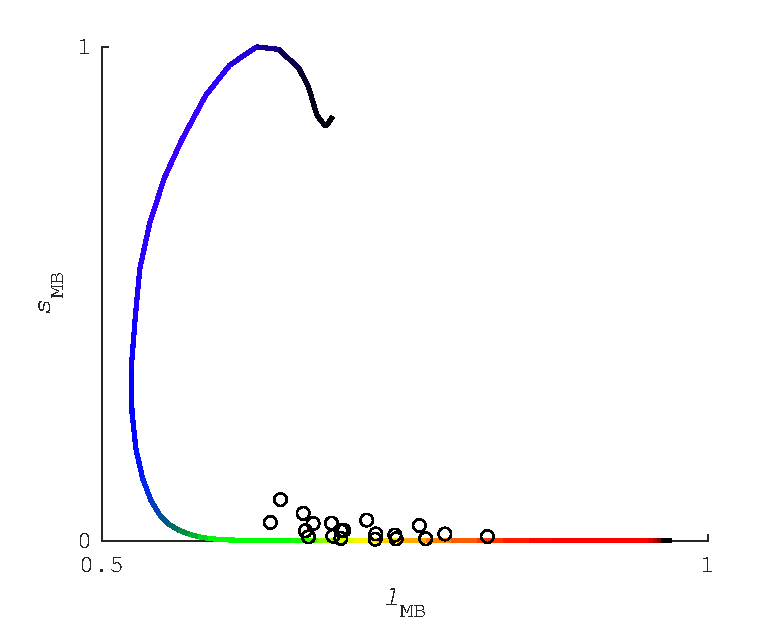
\includegraphics[max width=\textwidth]{figs/LitRev/ColorimetryDemo5.pdf}
\caption{A \gls{MB} chromaticity space diagram (as per \gls{CIE} 170-2:2015 \citep{cie_cie_2015}) showing the values for the macbeth colour checker patches under D65, as in previous figures.}
\label{fig:lrMB}
\end{figure}

\subsubsection{Correlated Colour Temperature}

The \acrfull{CCT} of an illuminant is defined by CIE 15.3:2004 \citep{cie_cie_2004-2} as follows:

\begin{itquote}{}
The temperature of a Planckian radiator having the chromaticity nearest the chromaticity associated with the given spectral distribution on a diagram where the (CIE 1931 standard observer based) u', 2/3v' coordinates of the Planckian locus and the test stimulus are depicted.
\end{itquote}

Whilst by this definition a light source of any chromaticity could be assigned a \gls{CCT}, as the distance between the Planckian locus and the test stimulus increases, the \gls{CCT} becomes a less meaningful descriptor. CIE 15.3:2004 \citep{cie_cie_2004-2} defines chromaticity limits on the maximum distance between the Planckian locus and the test stimulus, beyond which \gls{CCT} should not be used, which are described in Equation \ref{eq:CCTlim}.

\begin{equation}
\Delta C=\left[\left(u_{t}^{\prime}-u_{P}^{\prime}\right)^{2}+\frac{4}{9} \cdot\left(v_{t}^{\prime}-v_{P}^{\prime}\right)^{2}\right]^{1 / 2}=5 \cdot 10^{-2}
\label{eq:CCTlim}
\end{equation}

where $u^{\prime}_{t}, v^{\prime}_{t}$ refer to the test source and $u^{\prime}_{P}, v^{\prime}_{P}$ to the Planckian radiator.

Figure \ref{fig:BBR} shows Planckian locus (the curve formed by a set of black body radiators of different temperatures) in \gls{CIE} 1931 chromaticity space. It is worth noting that most real light sources (natural and artificial) fall upon the relatively straight section of the left-hand part of this line.

\gls{CCT} is often used as the independent variable in experiments, with the implicit assumption that this can be considered a complete descriptor of a light source. This assumption only holds to the extent that the spectral form is similar between conditions (for example if only a single light source is used and well defined filtration is applied, which shifts the chromaticity of the light source along the Planckian locus), and that the only difference between conditions is a shift along the Planckian locus. 

A shift in chromaticity perpendicular to the Planckian locus would result in no change to the \gls{CCT}. To counter this issue, an additional parameter ($D_{\text {uv }}$) is defined \citep{ohno_practical_2014} as per Equation \ref{eq:Duv}, which provides a value for the distance from the Planckian locus.

\begin{equation}
D_{\mathrm{uv}}=\left[\left(u^{\prime}-u_{0}^{\prime}\right)^{2}+\left(\frac{2}{3} v^{\prime}-\frac{2}{3} v_{0}^{\prime}\right)^{2}\right]^{\frac{1}{2}} \cdot \operatorname{sgn}\left(v^{\prime}-v_{0}^{\prime}\right)
\label{eq:Duv}
\end{equation}

where $\operatorname{sgn}(z)=1$ for $z\geq0$ and $\operatorname{sgn}(z)=-1$ for $z<0$.

\citet{ohno_practical_2014} notes that the combination of \gls{CCT} and $D_{\text {uv }}$ is suffice to describe the chromaticity of most light sources, and does so in a fashion which is slightly more intuitive than values of chromaticity.

\begin{figure}[htbp]
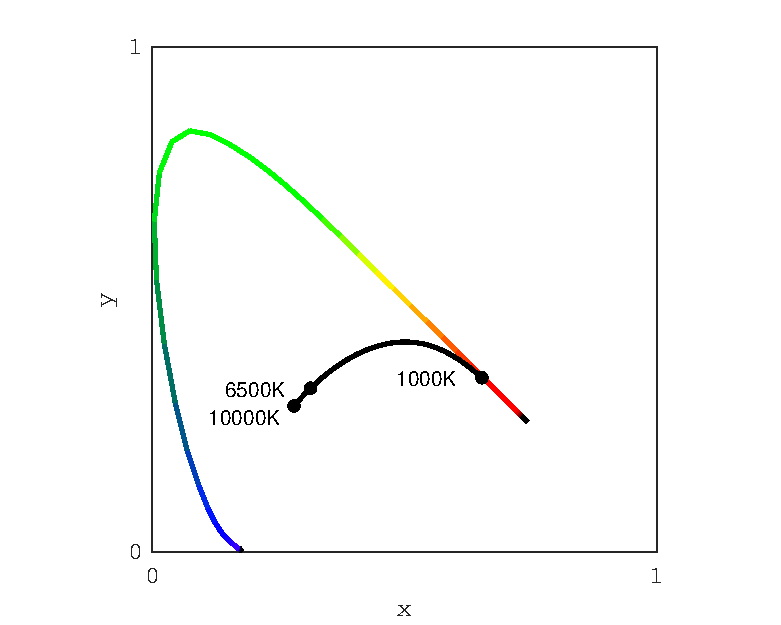
\includegraphics[max width=\textwidth]{figs/LitRev/BBR.pdf}
\caption{The Planckian locus on a \gls{CIE} 1931 chromaticity chart, highlighting \glspl{CCT} of 1000K, 6500K and 10000K.}
\label{fig:BBR}
\end{figure}

\clearpage
\subsection{Colour rendering}

Colour rendering indices provide an indication of the colour appearance of objects under a test illumination. Colour fidelity indices (properly a subset of colour rendering indices, however the most commonly used colour rendering index is in fact a colour fidelity index) are designed to describe how well a light source will produce a faithful appearance in terms of corresponding colorimetry to an appearance under \gls{CIE} D-series illuminant (daylight proxy) or a black body radiator. %Target values are generally provided in museum lighting guidelines \citep{ies_ies_1996,druzik_guidelines_2012,cibse_lighting_2015,thomson_museum_1986}. The recommended value for the ubiquitously used \gls{CIE} R\textsubscript{a} (As defined in \gls{CIE} 13.3:1995 \citep{cie_cie_1995}), often informally referred to as `CRI', varies from publication to publication, but is generally \gls{CIE} R\textsubscript{a}$>$80, but with no experimental work referenced to support this figure. 
Research in colour rendering is at a point of change and development, with the recognition that a single figure might never be enough to describe the complex, multidimensional, subjective and context dependent qualia of colour rendering\citep{rea_color_2008}. Thus new indices, and modifications and addenda to long-established indices are being proposed \citep{smet_memory_2012,davis_color_2010,rea_practical_2010,ies_ies_2015,teunissen_characterising_2016}.

If we were to take a bunch of balloons (or any objects, but balloons provide a simple and vivid image) of varied and multiple colours, from an area lit with daylight to an area lit with artificial light, and the colour appearance changes, for example the colours become more dull, we would generally be disappointed. In this case, we could say that we were dissatisfied by the colour rendering qualities of the artificial light source. If the colours remained the same we probably would think little of it, but if we were pressed for a comment, we might say that the colour appearance was satisfactory. 

If the balloons stayed the same colour as they had been under daylight, we would be witnessing a high level of colour fidelity (fidelity meaning faithfulness or truthfulness). If fidelity aligns well with the priorities of the user, then high levels of fidelity are desirable. If the appearance of the balloons had changed in some other way than becoming more dull - for example the colours became more vivid or the hue of certain balloons changed drastically, we might not neccessarily be disappointed, but this would still represent a situation where we were witnessing poor fidelity.

Generally when discussing colour fidelity, we are actually discussing fidelity to appearance under daylight or sometimes a Planckian radiator, aka a black body radiator. This is a fine comparison, but one which should be consciously considered; fidelity is not a measure of a light source per se, it is a comparison of that light source to a reference illuminant.

Fidelity has long been considered semi-analogous for colour rendering as a whole, but it is really only one element of colour rendering\footnote{Here I should point out that the \gls{CIE} definition of colour rendering, from the publication \gls{CIE} S 017/E:2011 ILV: International Lighting Vocabulary \citep{cie_cie_2011} reads: ``Effect of an illuminant on the colour appearance of objects by conscious or subconscious comparison with their colour appearance under a reference illuminant.'' You might notice the similarities to the definition I have ascribed to colour fidelity, and specifically not colour rendering. This is an unfortunate clash of nomenclature which I see as inappropriate usage on the part of \gls{CIE}, and at some point I hope this official definition will be updated to match the modern vernacular.}. When considering how `good' a light source is at facilitating colour with the objects which it illuminates, we might consider different measures alongside or in place of fidelity.

\begin{itemize}
\item \emph{Colour Fidelity (to recap)} - A measure of comparison between how colours appear under daylight (or other reference) and how they appear under another light source. %Do the balloons appear the same colour indoors and out? Are individual colours important or is an average suitably representative?
\item \emph{Chromatic Discrimination} - The ability of a light source to illuminate objects such that subtle differences in colour are made most visible. %Can you tell the difference between all the balloons? How big are the differences? Are threshold differences more or less important than the perceived magnitude of suprathreshold differences?
\item \emph{Observer Preference} - Subjective preferences for the colour of objects, potentially related to an increase in saturation, or an observer's memory of colours, or specific colour effects (e.g. increased saturation of skin tones). %Do the balloons look `nicer'/more vivid/more like the last time you saw them?
\end{itemize}

These areas overlap, and often exhibit correlation. For example, if a light source has properties which allow for high fidelity rendering, quite often that light source might also allow for good colour discrimination and also facilitate colours which might appear natural and/or pleasing. These are not reliable correlations however; it is quite possible to have a light source with very dissimilar properties to daylight that could score highly on discrimination and/or preference, or vice versa.

The index in widest use currently for quantifying colour rendering is \gls{CIE} R\textsubscript{a} (The General Colour Rendering Index). At the beginning of this doctoral project, this metric was used almost exclusively to generate the figure listed as `CRI' on the packaging for bulbs available commercially. %In the intervening time, IES RP-30-15 \citep{ies_ies_2015}, and more recently IES RP-30-18 \citep{ies_ies_2018}, have been published and have found considerable uptake from manufacturers.

\gls{CIE} R\textsubscript{a} is a colour fidelity metric, produced by computing the colour differences of 8 specified test colour samples (TCSs), between the situation where illumination is provided by the test source and that where it is provided by a reference illuminant with the same \gls{CCT} as the test source, and taking the arithmetic mean of these colour differences. The index is scaled such that the highest score is 100, for light sources which reproduce the TCSs under the reference illuminant exactly, with any light source which induces a colour shift receiving a value less than 100, descending below 0 if the magnitude of the shifts are great enough.

The most recent version of the standard specifying this metric is `\gls{CIE} 13.3-1995 Method of Measuring and Specifying Colour Rendering Properties of Light Sources' \citep{cie_cie_1995}. This document briefly overviews the history of, and necessity for, a colour rendering index and highlights areas of the procedure which vary compared to previous recommendations, and clearly details the recommended procedure. The process is summarised in the flow chart of Figure \ref{fig:criflow}. For a worked example see \citet[p.388]{hunt_measuring_2011}.

In response to a lack of confidence that \gls{CIE} R\textsubscript{a} delivered meaningful values for LED illumination, a considerable amount of research and discussion has revolved around the subject of a colour rendering index to supersede \gls{CIE} R\textsubscript{a}. This is commonly complicated by the incorrect assumption that the values obtained from a fidelity index in some way correlate with preference. A more valid criticism of \gls{CIE} R\textsubscript{a} is that it comprises deprecated methods and data sets for computing intermediary stages within the process of calculation, and thus this theoretically limits the `correctness' of any values produced by it.

Following many years where multiple \gls{CIE} technical committees aimed to deliver updated colour rendering indices, but subsequently didn't make any firm recommendations, an IES group was formed with the aim of examining the issue. The output of this IES group was the production of IES TM-30-15\cite{ies_ies_2015}, which follows the same philosophy as \gls{CIE} R\textsubscript{a} but with more modern colour science. It is still a contentious issue whether this updated index genuinely offers advantages over \gls{CIE} R\textsubscript{a}. 
% it also includes a bunch of other things...
% and IES TM-30-18?

Alternative propositions which offer fundamentally different approaches to the evaluation of colour rendering have been offered in recent years, including: 
\begin{itemize}
\item indices based on production of memory colours \citep{smet_memory_2012}.
\item indices which consider the size of the gamut of a TCS set \citep{rea_color_2008,teunissen_characterising_2016}.
\item indices which are fundamentally fidelity indices but which penalise or reward specific traits known to be disliked/preferred \citep{ohno_rationale_2010}.
\end{itemize}

\begin{figure}[htbp]
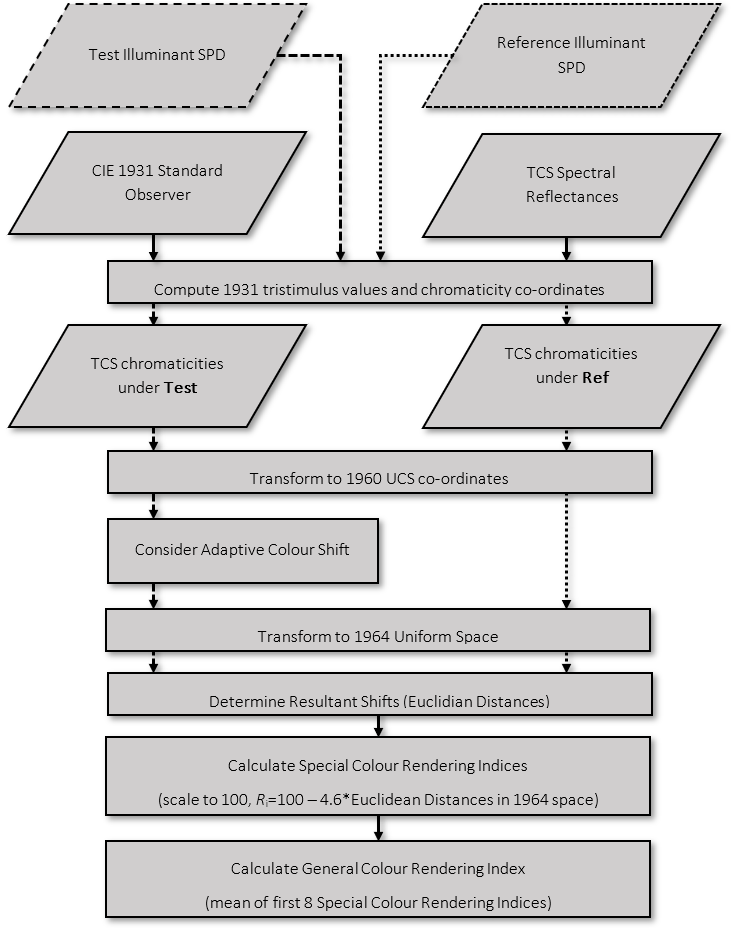
\includegraphics[max width=\textwidth]{figs/LitRev/criflow.png}
\caption{The stages of calculation for the computation of the \gls{CIE} General Colour Rendering Index. Notes: Reference illuminant: the same or nearly the same \gls{CCT}. Below 5000K reference spectrum will be that of a black body radiator, and from 5000K `one of a series of spectral power distributions of phases of daylight'.}
\label{fig:criflow}
\end{figure}

\clearpage

\subsection{Chromatic Adaptation and Colour Constancy}

\textit{Shortly after the start of my PhD program I attended a symposium for PhD students in the field of lighting research (LumeNet). At this symposium Prof. Michael Pointer delivered a welcome talk, and one particular part of it stuck with me.}

\textit{He described how at the start of his PhD studies \citep{pointer_colour_1972}, he had made copies of every paper which had been written on his subject (Chromatic Adaptation) which were available from the library, and written to any authors whose work he had been unable to access, requesting copies. At the end of his first year he had a binder which contained, as far as he was aware, everything ever written on the subject. He finished his story rather abruptly, along the lines of ``since then, so many people have written on the subject that it would take much longer than you have within a PhD program to read it all. I don't know what you all will do''. Not an encouraging thought!}

\textit{With this in mind, I shall attempt only to cover the basics and a few select papers of particular relevance in the following section, and shall take this opportunity to note my debt to a number of comprehensive overview papers, book chapters and theses on this subject: \citet{foster_color_2011,maloney_computational_1984,barnard_practical_1999,smithson_sensory_2005,hurlbert_computational_1998,brainard_color_2014,fairchild_color_2013}.}

\subsubsection{The problem}

At the start of this section I stated that ``Our perception of colour generally correlates with the way in which objects preferentially reflect some wavelengths over others''. It transpires that this ability is non-trivial, because our visual systems do not have access to the \glspl{SRF} of the objects which are seen, only the levels to which retinal cells are excited, which depends on the interaction of illuminant, surface and sensor. 

Figure \ref{fig:problem} demonstrates the problem, by reproducing Figure \ref{fig:1931} with a minor adjustment; where the previous figure had the chromaticities of the set of surfaces under only a single illuminant, a large number of illuminants are used here. It can be seen that it is not uncommon for one surface to have a chromaticity under one illuminant that another surface has under a different illuminant. Thus, the relationship between surface and chromaticity appears to break down.

\begin{figure}[htbp]
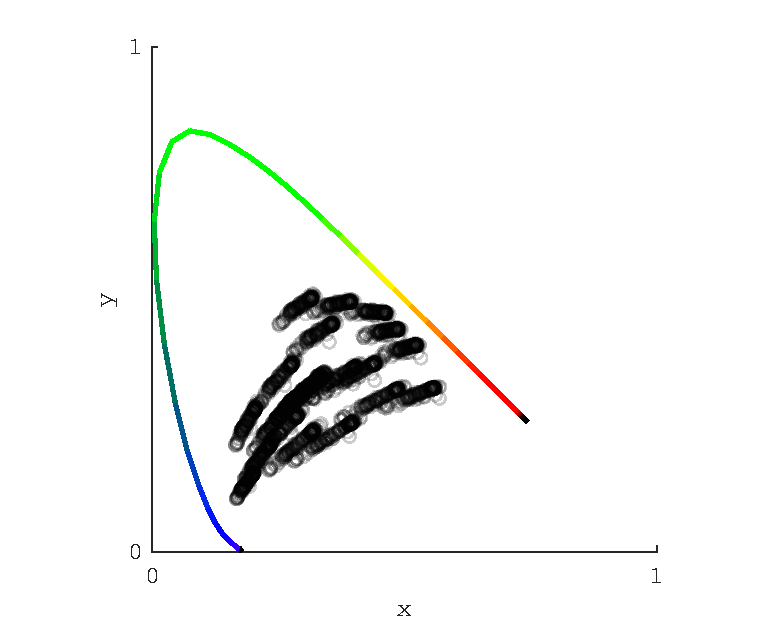
\includegraphics[max width=\textwidth]{figs/LitRev/ColorimetryDemo6.pdf}
\caption{A reproduction of Figure \ref{fig:1931}, but this time with the chromaticity co-ordinates for the 24 macbeth colour checker patches under a range of daylights, drawn from the Granada dataset \citep{hernandez-andres_color_2001} (further described in Section \ref{sec:coldata}).}
\label{fig:problem}
\end{figure}

In order to provide a representation of colour where the perceived colour remains constant across changes in illuminant (thus the term \emph{colour constancy}), the human visual system must find a way to solve this problem.

\subsubsection{Adaptation}

`Adaptation' is the general mechanism by which a finite range of sensitivity can be shifted within absolute sensitivity bounds. The benefit of having an adaptive system, as opposed to a fixed system, is that the sensitivity of the system to small changes is maximised, whilst maintaining a broad overall sensitivity, at the expense of being able to sense over the entire range at a single time-point. A visual demonstration of this is shown in Figure \ref{fig:Valeton} where it can be seen that that at a single level of adaptation (a single line) the range of intensity over which responses are generated is relatively small, but is extended through adaptation.

\begin{figure}[htbp]
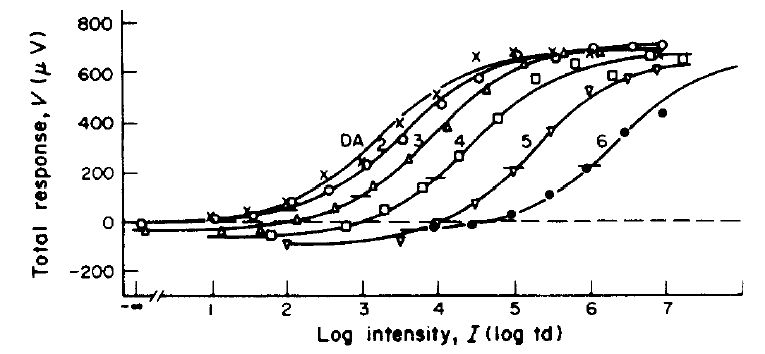
\includegraphics[max width=\textwidth]{figs/LitRev/Valeton.png}
\caption{Cone flash response at different levels of adaptation in macaques, reproduced from \citet{valeton_light_1983}. On the left `DA' stands for dark-adapted, with the rising numbers for the other lines relating to rising adapting levels.}
\label{fig:Valeton}
\end{figure}

In an environment such as the terrestrial environment, there is a great range in the level of illumination, but this range is rarely existent contiguously; levels of illumination tend to be similar across a scene, and only change rather slowly over time. The notable exception, and thus where we notice the expense of having an adaptive visual system, comes when we enter or exit an environment where illumination is almost entirely excluded, such as a dark cave or below-decks of a boat. 

Where the process of adaptation responds to overall illumination levels, it is referred to as light adaptation and dark adaptation. Where the process of adaptation responds to the wavelength composition of light reaching the eye it is referred to as chromatic adaptation.

In a natural environment, a change in the wavelength composition of radiation reaching the eye from a specific object might be caused by changing weather or time of day, or by the physical movement of the object from one space to another (where different lighting exists in the two different spaces). Figure \ref{fig:SPDnorm} shows a set of measured daylight \glspl{SPD}, normalised by luminance, showing that the wavelength composition varies quite considerably, though in a relatively systematic fashion.

\begin{figure}[htbp]
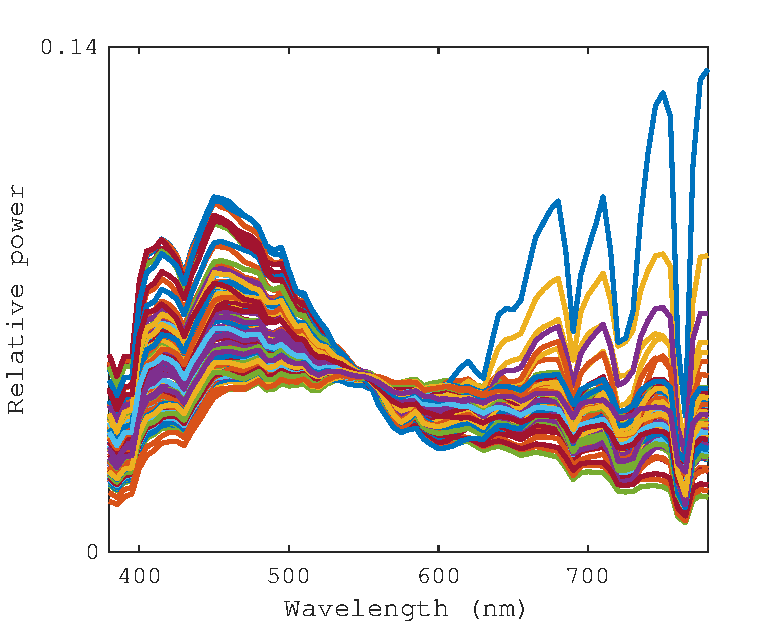
\includegraphics[max width=\textwidth]{figs/LitRev/ColorimetryDemo7.pdf}
\caption{The \glspl{SPD} of a subset of the daylight measurements of \citet{hernandez-andres_color_2001} (further described in Section \ref{sec:coldata}), normalised by luminance.}
\label{fig:SPDnorm}
\end{figure}

\subsubsection{Mechanistic vs. Inferential}

In the literature there seems to be a long-running grapple between colour constancy and chromatic adaptation, with blurred boundaries and mixed definitions occurring frequently. \citet{brill_chromatic_1986} drive a wedge between the two concepts, but refute the traditional division that chromatic adaptation is the process and colour constancy is the ability, asserting that the two should be considered as separate processes, operating on different timescales and in different fashions.

\citet{hurlbert_computational_1998} divides computational models of colour constancy into two classes: \emph{sensory} and \emph{perceptual}, which broadly follow the low-level / high-level divide. `Sensory' models `could be achieved early in visual processing by adaptive scaling of the initial receptor responses'. `Perceptual' models `would necessarily occur at later stages of visual processing'.

Hurlbert [personal communication] notes that understanding the differing perspectives of researchers from different fields allows one to understand how the mixed use of these terms in the literature may have arisen: 

\begin{itquote}{}
The mixed use of the terms chromatic adaptation and colour constancy is largely explained by different usages in different fields. In \emph{colour science}, chromatic adaptation is often considered synonymous with colour constancy, as it is considered to be the only mechanism contributing to stabilising colour appearance under changes in illumination. In \emph{vision science}, colour constancy is generally defined as a perceptual phenomenon, and distinction is made between different contributory mechanisms at different levels (which \citet{hurlbert_computational_1998} attempts to define and onto which different proposed computational solutions are mapped).
\end{itquote}

Within vision science, the most common use of the term `chromatic adaptation' now seems to be to refer to low level adaptation, with \citet{brainard_color_2014} using the term `mechanistic' to refer to this type of transformation.

\begin{itquote}
Adaptation of this sort supports constancy to the extent that its overall effect is to stabilize the post-receptoral representation of the light reflected from objects across changes of illumination (as well as other contextual changes).
\end{itquote}

The term `colour constancy', by contrast, is used to refer to higher level inference-based processes, which occur at faster timescales than are possible by adaptation alone \citep{rinner_time_2000}. It seems likely that multiple processes work in tandem at multiple levels and timescales to achieve colour constancy \citep{hurlbert_colour_2007}.



\subsubsection{Von Kries Adaptation}

The conceptually simplest model of chromatic adaptation, and the forefather of many other models, is that referred to as Von Kries adaptation.

Johannes von Kries was one of the first to deeply consider chromatic adaptation, and appears to have understood it as a problem of sensory adaptation. In his formative series of papers, available in translation \citep{von_kries_beitrag_1970}, he laid out how the study of chromatic adaptation could be divided into two broad and complementary aims. 

The first referred to the systematic representation of the transforms in sensation caused by specific adaptations, such that \textit{``for any light mixture stimulating the readapted part [of the retina], another light mixture is specified that stimulates the same sensation in a normally adapted part \dots The purpose of this study would be solved completely if a general rule could be obtained for the effects of all possible adaptions.''} The search for `corresponding colours' (pairs of colours which match under asymmetric adaptation states), and for suitable systems to predict the appearance of colours in all situations, fall within this category of exploration. Out of this aim grew the study of \glspl{CAT}, where the search for an algorithm which would mathematically predict the locations in colour space of corresponding colours has been the fundamental goal \citep{cie_tc_1-52_cie_2004}.

Von Kries suggested that the second categorical aim of chromatic adaptation research ought to be to discover `how the adaptation is produced by exposure to any particular color, continued over an extended period of time.' 

Von Kries' distinction carves a divide between the study of the mechanisms of chromatic adaptation, and the effects of chromatic adaptation. It would be unreasonable to think of these areas of study as unrelated, but it seems reasonable to recognise their separability. 

%In the same set series of papers, von Kries laid out his understanding of chromatic adaptation, in terms of both how corresponding colours might be calculated, and how one might consider the underlying mechanisms which allow for colour constancy to operate. Here I shall abridge some of his writings to present the most salient insights, and attempt to explain what is meant by a `von Kries transform' in modern parlance.

Von Kries noted that `light mixtures that appear matched to the white-adapted eye always remain matched to the eye when it is adapted in any other manner.' This is known to be only partly true; if referring to photopic vision solely (where rods are bleached and cones provide the basis for vision). The implication of this statement is that the spectral sensitivities of the cone cells do not change as a result of chromatic adaptation. If they were to change in some way, then distinct mixtures of light which match in one adaptive state might fail to match under a different state. Von Kries referred to this idea as the `persistence rule.'

The second rule which von Kries presents is referred to as the `theorem of proportionality'. This theorem claims that when two pairs of corresponding colours (colours A and B under illuminant 1, and colours C and D under illuminant 2) are additively combined (A with B, and C with D), the resulting colours will also be corresponding colours. It follows from the von Kries' theorem of proportionality that increasing or decreasing the luminance of corresponding stimuli shouldn't void their equality, though of course this statement relies even more heavily on the caveat that this should only be assumed for photopic vision.

Von Kries goes on to suggest that it also follows that, if considered in combination with Grassmann's law \citep{grassmann_zur_1853}, the conversion of any arbitrary light by exposure to conditions causing a specific chromatic adaptation can be known if the nature of three other conversions are known. This relies on it being possible to consider any light as a linear combination of three others, and for the mechanism of chromatic adaptation to depend solely on the fatiguing of three independent systems.

Von Kries' assertions may be mathematically described as:

\begin{subequations}
\begin{align}
L_{a}&=K_{L}L \\
M_{a}&=K_{M}M \\
S_{a}&=K_{S}S
\end{align}
\end{subequations}

where $L$, $M$ and $S$ represent the cone group responses; $K_{L}$, $K_{M}$ and $K_{S}$ represent distinct scalars and $L_{a}$, $M_{a}$ and $S_{a}$ represent the post adaptation cone group responses\footnote{This specific notation is taken from \citet[p. 183]{fairchild_color_2013}.}. In terms of what might set these scalars, or gain values, von Kries suggested that: 

\begin{itquote}{von_kries_beitrag_1970}
the organ of vision becomes less effective for that kind or for that part of its performance which is demanded from it for an extended period of time, whereas it becomes more effective for the activity which is, in a sense, opposed to that. This can be conceived in the sense that the individual components present in the organ of vision are completely independent of one another and each is fatigued or adapted exclusively according to its own function.
\end{itquote}

Many interpretations have been made of this statement, and a corresponding number of nominations for methods by which to calculate values of $K$ have been proposed. The most frequently considered methods are those referred to as \acrfull{GW} (where the reciprocal of the mean response across a scene is used) and \acrfull{BiW} (where the reciprocal of the brightest point in the scene is used). \citet{finlayson_shades_2004} showed that these two variants can be considered as part of a single framework (Minkowski norm), and that other members of this family of algorithms provide benefits over \gls{GW} and \gls{BiW}.

Von Kries' thoughts have inspired many decades of research into \glspl{CAT}, which are a vital part of modern colour appearance models and other colour science computations, such as colour rendering index calculations. This relatively simple concept has remained relevant, as noted by \citet[p. 182]{fairchild_color_2013} who reproduces this quote:

\begin{citequote}{von_kries_beitrag_1970}
If some day it becomes possible to distinguish in an objective way the
various effects of light by direct observation of the retina, people will perhaps
recall with pitying smiles the efforts of previous decades which
undertook to seek an understanding of the same phenomena by such
lengthy detours.
\end{citequote}

followed by the comment:

\begin{citequote}{fairchild_color_2013}
Over eleven decades later, there is no one looking back at von Kries' work
with a ``pitying smile''. Rather, many are looking back at his work with
astonishment at how well it has withstood the test of time.
\end{citequote}

\subsubsection{Retinex}

Considered in the context on von Kries' work, the Retinex model of Land et al. \citep{land_retinex_1964,land_lightness_1971,land_recent_1983,land_recent_1986,mccann_quantitative_1976} might be described as `Von Kries adaptation with spatial considerations' but I imagine such a statement would have rather riled the often bombastic sounding Land. It appears to have been Land's understanding that the Retinex model was not a model of chromatic adaptation, but rather a model to usurp and do away with the very concept of chromatic adaptation (Land's papers on the subject \citep{land_retinex_1964,land_lightness_1971,land_recent_1983,land_recent_1986} do not once use the term `chromatic adaptation', nor is the work of von Kries ever explicitly referred to). 

Land was fond of picking apart Newton's statements regarding colour; particularly that the perception of colour was the result of an objects' `excess and predominance in the [spectra of the] reflected light' \citep{newton_opticks_1704}. Land asserted that rather than work from the premise that the visual system was correcting an absolute record of the world, by normalising it to account for the ambient light source, one should instead consider visual input only as a relative record, where each element within a scene only takes on properties by comparison with the other elements of the scene. 

He suggested for consideration the idea of the human visual system recording three separate lightness images, each representing the recording from a different band of receptors, where each element within each image is scaled against the brightest element in each specific image. Retinex theory also provides an interesting algorithm for discounting not only coloured illumination but illumination which varies across the visual field.

However, \citet{barnard_practical_1999} points out that the various versions of the Retinex algorithm simplify to versions of the Von Kries adaptation, and \citet{brainard_analysis_1986} found that `the algorithm is too sensitive to changes in the color of nearby objects to serve as an adequate model of human color constancy'. In addition, it has been found to be computationally difficult to implement, with no clear way in which it could be biologically implemented (though see \citet{hurlbert_formal_1986}).

The work of Land et al. has spurred a great deal of progress in the world of digital imaging, where the term `computational colour constancy' is used. The number of distinct algorithms increases at a rate which seems to always accelerate, and I shall not review them all here, though I shall point to valuable overview papers:  \citet{hordley_reevaluation_2006, gijsenij_computational_2011, hurlbert_computational_1998}.

\subsubsection{Linear models}

If we extend the common interpretation of colour constancy (that colours should remain constant), to a stricter case where we actively try to recover the \glspl{SRF} of surfaces, simple Von Kries-type transformations no longer suffice. \citet{maloney_physics-based_2001} and \citet{yang_illuminant_2001} discuss what they term the `RGB heuristic'. Simply put - this is the commonly held assumption that a set of cone catches under one illuminant will be related to a second set of cone catches under another by a transformation which can be fully described by the chromaticities of the illuminants. As \citet{maloney_physics-based_2001} says `there is no \emph{mathematical} reason to expect [this] to hold, even approximately'. This can be considered from the perspective of colour rendering; it is known that objects which are metamers under one illuminant might not be under another. This renders simple models of colour constancy ineffective. \citet{foster_frequency_2006} quantified the frequency of metamerism in real scenes and found it to be `sufficiently large to affect visual inferences about material identity'.

For this stricter definition of colour constancy Maloney et al. \citep{maloney_computational_1984, maloney_color_1986} propose a method which makes use of discrete linear models, whereby the set of real \glspl{SRF} and real \glspl{SPD} are approximated by a small number of fixed basis functions. 

\citet{maloney_color_1986} find that `with three classes of photoreceptors, we can exactly recover surface reflectances drawn from a fixed model of surface reflectance with at most two degrees of freedom'. \citet{maloney_computational_1984} showed that this generalised such that with $n$ classes of photoreceptors, \glspl{SRF} could be reconstructed for surfaces drawn from models with $n-1$ degrees of freedom, so long as there were not more than $n$ degrees of freedom in the illumination model, and so long as the minimum complexity condition was met (there were enough surfaces visible).

Despite its mathematical elegance, quantitative analysis of this algorithm showed that its performance was poor \cite{brainard_bayesian_1994, finlayson_color_1995}, which is not surprising considering that natural surface \glspl{SRF} generally require more than two basis functions for accurate reconstruction.

\bigskip

There are many further ideas, theories, and concepts relating to colour constancy and chromatic adaptation which are beyond the scope of this chapter, but that the reader may find of interest: gamut mapping algorithms \citep{forsyth_colour_1990,forsyth_novel_1990,forsyth_colour_1989,finlayson_color_1996}, bayesian colour constancy \citep{finlayson_color_2001, brainard_bayesian_2006,gazzaniga_bayesian_2009, brainard_bayesian_1994,gehler_bayesian_2008} and specular-reflectance-based algorithms \citep{mollon_monge_2006, morimoto_discrimination_2018,hurlbert_computational_1998}.

%% Removed stuff ---------------------------------


%Colour constancy refers to the stable perception of object colour appearance, in spite of a change in illumination which would cause a change in the nature of the stimuli reaching an observer\footnote{The terms `chromatic adaptation' and `colour constancy' are often used interchangeably; within this thesis I shall use `chromatic adaptation' to refer to an adaptive mechanism, and `colour constancy' as the ability possessed by an organism. For a discussion of the distinction of chromatic adaptation and colour constancy see \citet{brill_chromatic_1986}}. This objective change in stimuli seems to be effectively but not completely discounted by the human visual system; in order to maintain a stable perception of object appearance. 

%If however, one asked an observer whether the \emph{appearance} of an object has changed between the two conditions, the observer would generally say that it has. To some extent, we seem to have access to both the `raw input signals' and some estimate of the underlying \gls{SRF}.


%It is the popular understanding that when the illumination changes, the colour of an object (to use the term `colour' in its vernacular form, as representing an object attribute) does not change. This understanding holds true for all but the most extreme artificial illuminations, such as very narrow-band illuminantion. 


% \begin{figure}[htbp]
% 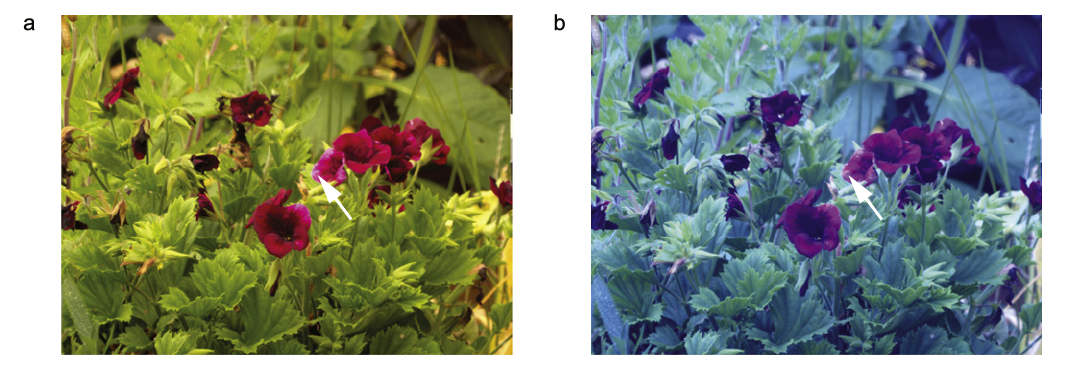
\includegraphics[max width=\textwidth]{figs/LitRev/fosterflowers.png}
% \caption{A single scene under two illuminants (\Gls{CCT} = 4000k and 25000K), reproduced from \citet{foster_color_2011}.}
% \label{fig:fosterflowers}
% \end{figure}

% \begin{figure}[htbp]
% 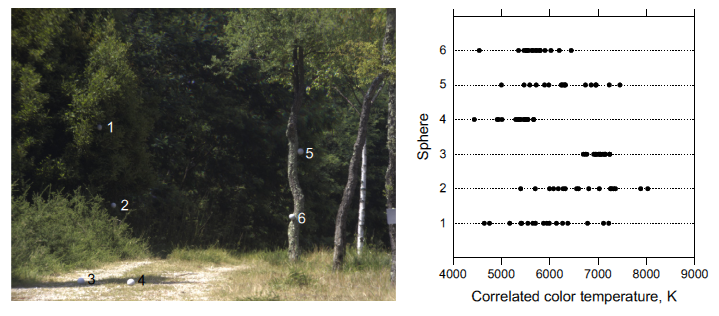
\includegraphics[max width=\textwidth]{figs/LitRev/greyballs.png}
% \caption{Reproduced from \citet{nascimento_spatial_2014}. Original figure caption: ``The color rendition on the left shows the scene with six embedded probe spheres indicated by numbers. The dot plot [on the right] shows the distribution of the CCTs of the local illumination at the 17 sample points on each of the spheres.''}
% \label{fig:greyballs}
% \end{figure}

%Figure \ref{fig:greyballs} gives an indication of the extent to which an object (or more precisely in this case, a group of nominally identical objects) can have varying colorimetric attributes across relatively minor spatial variation. 
%KC: This reads oddly to me, as it's more the illuminance that's varying than the object (if I've understood?).  I'd rephrase this.

% \begin{figure}[htbp]
% \includegraphics[max width=\textwidth]{figs/LitRev/X.png}
% \caption{\hl{Figure showing variation over time.}}
% \label{fig:X}
% \end{figure}

% Figure \ref{fig:fosterflowers} shows a single scene under illumination of two different \glspl{CCT}. The appearance of the object under the two illuminants is likely to have remained somewhat stable to an observer within the real scene, with observers choosing similar colour names for the object under each condition\footnote{Of course the appearance here, with these two images side-by-side, highlights the differences between the two conditions, and shows that under a single state of adaptation there is a clear distinction.}. 


% \subsubsection{Can chromatic adaptation fully account for colour constancy?}

% It may at first appear as though chromatic adaptation may be able to fully account for colour constancy

% RGB heuristic
% yes - cornsweet
% mechanistic vs inferential


% A similar level of variation occurs across time, for example as the sun passes behind a cloud.

% And so we have the central problem of colour constancy and chromatic adaptation: objects of which we have stable colour perceptions are able to be variant in both radiometric and colorimetric attributes without losing their apparent stability. The study of colour constancy aims to answer many questions which revolve around this central conundrum.

% Traditionally %(pre-1986, when \citet{arend_simultaneous_1986} performed what \citet{foster_color_2011} refers to as `the first systematic behavioral experiments' on color constancy) 
% there have existed two stances regards the nature of colour constancy; one held that it was enabled by adaptation of the sensory system, and the other that it was the result of unconscious inference. %KC: citation required
% It is my understanding that whilst great progress has been made in the intervening three decades, this is still a central question, although it appears to be widely accepted that the two frameworks might be complementary rather than mutually exclusive. %KC: citation required

%The best justification for their separation is perhaps that success in their study might serve different aims. 
%The first, the prediction of colour appearance, serves to further the utility of colour science, in particular colour appearance modelling, and the other systems which rely upon colour appearance modelling, such as colour difference formulation. 
%The second is best considered a vision science problem, concerned as it is with the function of the human visual organ, and advancement might endow us with an extension in our understanding of the human body. This in turn would have benefit in multiple areas, including feeding back to the prior aim, for once we understand the underlying mechanics we stand a much better chance of creating robust predictors of colour appearance. 
%Of particular interest to this author, understanding the underlying mechanisms of colour constancy should allow for a more intelligent design of lighting for the spaces which we inhabit, considering that artificial lighting need only resemble natural lighting to the extent that the visual system treats it as similar enough. Creating a colorimetric match to a specific spectra such as D65 is relatively easy, but until chromatic adaptation is more thoroughly understood it is not necessarily entirely clear what the appearance of such a match, or objects illuminated by it, might be. 

%The investigation of \glspl{CAT} generally occurs through the fitting of algorithms to data of corresponding colours, collected in varying manners, such that corresponding colours might be predicted for specific situations. The principal divides between the types of \gls{CAT} tend to hinge upon the method used to collect the data. \citet{nayatani_development_2006} divides the set as those derived from chromatic adaptation theory and those derived from fitting to experimental data, whereas Luo44 makes the divide between those studies based on aperture based experimental procedures and non-aperture based experimental procedures (which generally incorporate more complex, and therefore arguably more realistic, stimuli). Both parties use the terms `CAT Type I/II' to refer to these distinctions, but it is not entirely clear whether their distinctions are complementary. 

% This duality %get rid of this bollocks
% is mirrored by Foster37 in his discussion of the experimental methods employed in colour constancy research where he describes fundamental differences between those experiments which probe chromatic adaptation by asking observers to make `paper matches' (make it look like these two patches were cut from the same sheet of paper) and h/s/b matches (where observers are asked to match appearance in a non-relational manner, that is to match the qualia of a stimuli). This duality occurs again in Foster's37 comparison of relational and non-relational colour constancy, where relational refers to the maintaining of colour relationships in a scene and non-relational again refers to abstracted stimuli qualia). It is my suspicion that all of these disparate dualities are representations of the fundamental duality considered at the beginning of this chapter; that of a distinction between sensory adaptation and inferential computation.

\subsection{Experimental Methods for Colour Constancy Research}

A large range of experimental methods have been used to investigate the problem of colour constancy, partly because different experimenters were approaching the problem from different angles aiming to accomplish subtly separate goals.
Those approaching from a mathematical angle (perhaps with the mind-set `if we find the algorithm which predicts corresponding colours a- this is very useful for industry and b- we can then work backwards to explain how human colour constancy may occur') are concerned primarily with producing chromatic adaptation transforms.
Those approaching colour constancy with a basic interest in the physiology and general function of colour constancy have adopted/created a rather wider set of experimental techniques, owing to the fact that this direction of study is much less well defined than the former, and is at a more exploratory stage of its development.
The \gls{CIE} TC 1-52 report (\gls{CIE} 160:200442) includes an interesting note on the distinction between these two broad approaches; an appendix discusses the reasons why a concerted recommendation was not reached by the group lists the principal factor being a distinction between perspectives as described above. 
\gls{CIE} TC 1-5242 and Luo44 provide a comprehensive overview of the different methods which have been used by the CAT group:
1.	Haploscopic matching
2.	Local Adaptation Matching
3.	Memory Matching
4.	Magnitude Estimation
Haploscopic Matching is the most common technique in this field, and the term refers to experiments which differentially adapt the two eyes and allow an observer to vary attributes of the stimulus presented to one eye such that it in some way matches the attributes of a fixed stimulus shown to another eye. Whilst this is in many ways unnatural, the benefits are that an experiment can be set up so that there is no time interference (the presentations are simultaneous, so memory effects are avoided) and that high precision of match is relatively easily achieved. As assumption is made that the adaptation of each eye is independent.
 
Figure 11 From42.
Local Adaptation Matching can be considered as a variation of haploscopic matching where instead of differing adaptational stimuli being presented to each eye, differing adaptational stimuli are presented to different parts of the same eye (spatially distinct areas of the same retina). The assumption here is that there is minimal intra-retinal interaction. MacAdam's 1956 study49 epitomises this technique. This experimental technique requires that observers minimise eye movement, in order to maintain spatially distinct adaptation.
Memory Matching has traditionally been performed by training observers to communicate colour sensation through the munsell system notation50,51, and then asking observers adapted to different ambient lighting to describe set real objects using such notation. This technique is not much used due to many limitations and confounding factors. Luo44 details the limitations  of this experimental technique succinctly: `a substantial training period being required, complicated procedures for data analysis, lower precision than that of haploscopic technique, limited capacity for retaining information, and memory distortion.'
Magnitude Estimation appears to be similar to memory matching, in that observers are requested to verbally describe an object whilst in an ambient adapting field. The distinction is that the observers are requested to communicate their perceptions using the perceptually meaningful attributes of hue, saturation and brightness, and as such results can be easily integrated into colour appearance models. Recent experiments52,53,54,55,56,57 collected data which was used to create CIECAM97s.
Away from the development of CATs, a subtly different set of experimental techniques has been developed with which to probe the operation of colour constancy. An admirable overview is provided by Foster37:
1.	Asymmetric Matching
2.	Colour Naming
3.	Achromatic Adjustment
4.	Discriminating Illuminant Changes from Reflectance Changes
Asymmetric matching is in many ways synonymous to the haploscopic matching described above and by in \gls{CIE} 160:200442, in that it describes an experimental set-up whereby one stimuli is compared with another, generally where each stimuli exists within a distinct adapting field and attributes of one stimuli can be either adjusted or responded to by an observer. The term asymmetric matching might be thought to be inclusive of a wider range of experimental set-ups, where haploscopic (Greek roots: haploieides, single and skopeo, to view) is necessarily concerned with each individual eye receiving distinct input. Asymmetric matching may refer to experiments where stimuli are viewed simultaneously, successively, or in an alternating fashion, binocularly or haploscopically.
Colour Naming is a technique employed with the aim being a more natural task than  asymmetric matching, and removing some of the `instruction effects' probed by Arend and Reeves40. Foster argues37 that colour naming represents a task apt to measure colour constancy more directly, as opposed to the `relational colour constancy' often studied in asymmetric matching experiments, since it concerns identification rather than equivalence. One clear benefit seems to be that the observer needn't be aware of the equivalence; it is expected that in such experiments there will be only one stimulus, perhaps with a temporally variant adapting field. An observer is simply asked to name colours, and this should theoretically result in a measure of adaptational colour constancy as opposed to inferential colour constancy, so long as the stimuli is suitably abstract . Colour names may be of a fixed set, or an observer may be given free choice. Analysis of results can employ a naming centroid based approach or a boundary focused approach. Speigle and Brainard58 proposed a novel approach combining magnitude estimation and colour naming with the aim to improve precision of response.
Achromatic Adjustment experiments ask an observer to in some way set a stimulus to a neutral achromatic tone, on the assumption that the internal grey point of an observer shifts in response to different adapting fields. These adjustments are generally easy for an observer to make, but the extrapolation of the results makes various assumptions about conceptual colour space and the nature of achromacy. Experiments are easily confounded by complex or real stimuli where there exists a close-to-neutral object in the scene which could consciously or unconsciously be used as a reference.
Discriminating illuminant changes from reflectance changes provides a key way to examine colour constancy in an operational manner. Following the assumption that chromatic adaptation allows an observer to discount the illuminant in some manner, an experimental set up where observers are requested to distinguish between an illuminant change and a reflectance change represents a situation which very closely mirrors the natural process of colour constancy. This experimental technique is well placed to examine whether or not colour constancy in this form is active and efficient, but it provides little way of probing the underlying mechanisms of colour constancy.

%recent advances in colour constancy?
% using more realistic stimuli
% the grey edges algo
% the comparison of grey edge and grey world/bright is white
\subsection{Illuminant and Surface Data Sources}

A useful guide to some of the existing datasets has been provided by \citet{kohonen_databases_2006}, though many of the links have rotted since publication, some new datasets have become available, and some datasets that weren't included have become known to me. In this section I shall describe the datasets available for use in studies such as this.

\subsubsection{Daylight datasets}

It is standard practice (see for example \citet{barrionuevo_contributions_2014}) to use illuminants generated from from CIE D-series formulae (see \gls{PTB} function `GenerateCIEDay') which are derived data collected by \citet{judd_spectral_1964}. Whilst the D-series provides a good approximation of daylight spectra, empirical data better represents any link between chromaticity and luminance, and any bias in the likelihood of occurrence of one spectrum over another. It is thought that the original data of Judd et al. is no longer available \citep[p.~60]{maloney_computational_1984}. The first three principal components of the data are available through \gls{PTB} as `B\_cieday'.

\paragraph{Granada Data.}
The Granada daylight database \citep{hernandez-andres_color_2001} contains 2600 measurements of daylight taken over the course of two years at a single site in Granada, Spain. Data is recorded for 300-1100nm with sampling interval of 5nm.\footnote{This data has been made available at \url{http://colorimaginglab.ugr.es/pages/Data}}

\paragraph{Other sources.}

The Parkkinen and Silfsten data described by \citet{kohonen_databases_2006}\footnote{Available at \url{http://cs.joensuu.fi/spectral/databases/download/daylight.htm}} comprises 14 measurements of daylight from afternoon and evening. The wavelength range is 390nm - 1070nm, with 4nm intervals.

The other potential sources of data, in addition to the \citet{judd_spectral_1964} data, do not seem to be currently available, but for completeness I provide them here: \citet{condit_spectral_1964, tarrant_spectral_1968, dicarlo_illuminant_2000, taylor_distribution_1941, henderson_spectral_1964, sastri_typical_1968, dixon_spectral_1978, sastri_spectral_1966,williams_statistical_2009,bui_group_2004}.

There are two authoritative reference books on the subject: \citet{henderson_daylight_1970,henderson_daylight_1977} (first and second editions) and \cite{robinson_solar_1966}. Also of interest may be \citet{minnaert_light_1993} (various editions), and \citet{lynch_color_2001} (various editions).

Two further datasets which are available only upon request are held by Dr Andrew Smedley of The Univesity of Manchester (320nm to 2800nm, since 2010, data collection ongoing) and Marina Khazova of Public Health England\footnote{Minimally described here: \url{https://uk-air.defra.gov.uk/research/ozone-uv/uv-uk-monitoring}} (350nm - 830nm, 1nm interval). It is hoped that these datasets may be made openly available at some point in the future.

Data specifically for dawn and dusk (with a small amount of data extending into what could be considered `daylight' is available from \citet{spitschan_variation_2016} as open access supplementary material from the journal publisher. 

An interesting additional source of data may be the work of \citet{peyvandi_colorimetric_2016}, who simulate a very large number of daylight, sunlight and skylight spectra. 

Finally, there is also a large corpus of information specifically about the light conditions in forest environments, although I have not yet had opportunity to investigate whether collected datasets have been made available \citep{sumner_catarrhine_2000,chiao_characterization_2000,federer_spectral_1966,geiger_climate_2003,thery_forest_2001,xu_changes_2013,wang_real-time_2006,endler_color_1993,brinkmann_light_1971,de_castro_light_2000,freyman_spectral_1968,fassnacht_review_2016,blackburn_seasonal_1995}.

%hutchison_relighting_2009

\subsubsection{Surface Reflectance datasets}

\paragraph{Krinov data.}
The Krinov data was originally published in 1947 \citep{krinov_spektralnaya_1947}, though it is now mainly accessed through a Canadian translation published a few years later \cite{krinov_spectral_1953}. It has recently been made available through \gls{PTB} \cite{brainard_psychophysics_1997} (as sur\_krinov.mat), and forms part of the SFU dataset \cite{barnard_data_2002}. It consists of 370 measurements of natural surfaces, measured at 9 locations around the USSR. It includes a large number of repeated measures (generally of objects at different angles), and has many measurements of objects which might be described as `background' surfaces rather than objects per se (e.g. soil, sand, turf). Measurements are available at 10nm sampling interval, mostly between 400 and 650nm, with some extending as far as 900nm, and some without data at parts of the range. The \gls{PTB} version of the data is a reduced set of 191 measurements, having excluded a number of measurements of various types of grass. 

\paragraph{`Natural Colors' data.}
The `Natural Colors' data \citep{parkkinen_spectral_1988} was collected to allow investigators to explore how well reflectances could be represented by low dimensional models\footnote{It is available at: \url{http://www.uef.fi/web/spectral/natural-colors}}. The data consists of 219 reflectance spectra of different leaves and flowers, between 400 and 700nm with interval of 5nm. It has recently been made available through \gls{PTB} (as sur\_koivisto.mat).

\paragraph{Vrhel et al. data.}
The \citet{vrhel_measurement_1994} data in its complete form comprised measurements of 64 Munsell chips, 120 Du Pont paint chips and 170 natural and non-natural objects. Similarly to the `Natural Colors' data, this data was again collected to allow investigations into the dimensionality of natural refelctance functions. The authors noted that they aimed to improve upon the Krinov data by decreasing the sampling interval (to 2nm), increasing the range of objects measured (and focusing on more object-like objects as opposed to background objects) and increasing the sampling range (to 390-730nm). To my knowledge only part of this set is currently available, as the FTP server referenced in the original publication is no longer accessible. The object reflectances alone are available through \gls{PTB} (as `sur\_vrhel.mat').

\paragraph{Standard Object Colour Spectra Database for Colour Reproduction Evaluation (SOCS) data.}
This international standard \citep{tajima_development_1998,iso/tc_130_graphic_technology_iso/tr_2003} collates more than 50,000 spectral reflectances of a wide range of type of surfaces, grouped into several categories. The database was originally created in order to allow for the assessment of colour reproduction of image input devices. Unfortunately, this data proves very difficult to access, and as yet I have been unable to assess it.

\paragraph{NASA data.}
The NASA data-set \citep{david_e._bowker_spectral_1985} comprises 156 measurements of different terrains and materials, presented to aid in the design of remote imaging systems to optimally detect surfaces of interest and to detect changes over time in these surfaces where this is of interest (e.g. changes in spectral signatures that reveal growth or disease of specific crops). Data was not collected by the authors, but digitised from 58 different sources, and so range and interval are not consistent throughout the set. Whilst the authors seem to have devoted a great deal of energy and care to accurate digitisation, `digitisation' seems to be limited to the printing of tabulated values rather than provision of digital files (we've come a long way since 1985) and so any use of this data may need to start with an extended period of careful transcription. The surfaces chosen for this set are sensibly biased towards those of interest to remote sensing applications, and so use of this data in vision science would likely require careful consideration. It is expected that there may be other similar datasets tailored to the needs of remote sensing which may be available, should this type of data be appropriate.

\paragraph{Foster et al. hyperspectral images}
The hyperspectral images of \citet{nascimento_statistics_2002,foster_frequency_2006} provide nominal \glspl{SRF} for full natural and suburban scenes. This data is valuable and rich in many ways. 

Notably, it can begin to represent the ubiquity/rarity of certain types of reflectances in the natural world, whereas the statistical distribution of surface variability in the abstracted databases so far considered is at the mercy of the collator. As Maloney puts it: ``in sampling spectral reflectances, we weight each spectral reflectance by its frequency of occurrence under whatever selection procedure we choose'' \cite{maloney_computational_1984}.

Additionally, the spatial inter-relationships between surfaces can be considered, which may be of particular value in trying to understand how an organism might operate under real-world conditions.

\begin{figure}[htbp]
    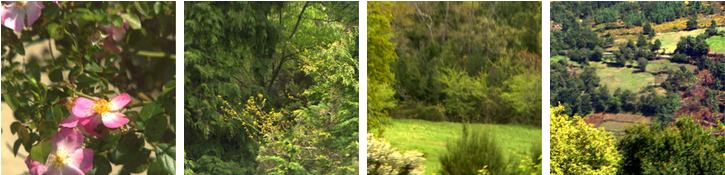
\includegraphics[max width=\textwidth]{figs/LitRev/Foster.png}
    \caption{A visualisation of the hyperspectral data for the first four images of the \citet{nascimento_statistics_2002} data. The other four available images are of non-natural environments.}
    \label{fig:Foster}
\end{figure} 

%In many ways hyperspectral images represent the ideal data for this type of experiment. They are much more closely linked to the real-world challenges faced by the human visual system in terms of statistical and spatial distribution of reflectances than data comprising abstracted spectral reflectances of a selected range of sampled surfaces. The statistical distribution of surface variability in an abstracted database is at the mercy of the collator, as Maloney puts it: ``in sampling spectral reflectances, we weight each spectral reflectance by its frequency of occurrence under whatever selection procedure we choose''\cite{maloney_computational_1984}. Of course the individual scenes still need to be selected in some way, with implicit assumptions about the goals of the human visual system being baked in at this stage (for example - should scenes include grassy landscapes and flora, trees laden with fruit, predators in hiding or human skin tones?).
%Using two-dimensional images would also allow for more advanced chromatic adaptation models to be considered, such as the group of algorithms based on Weijer et al.'s `Grey Edge' ideas \cite{weijer_edge-based_2007}. 

However, caution must be taken when using such data; whilst the hyperspectral images available are nominally `reflectance' images, the way in which reflectance is computed may make them unsuitable for some uses. Reflectance is estimated from radiance images by assuming uniform illumination across the scene, which for some use cases may be a particularly problematic simplification. %This is an acceptably minor distinction for many use cases, but in this specific case this introduces error in precisely the place where it needs to be avoided. In considering the effectiveness of chromatic adaptation transforms the goal is to separate the effect of variable reflectance functions from variable power distributions, and the ability to do this is hindered if an element of the power distribution variability is baked into the reflectance functions.

One final dataset which is worth mentioning, but which does not currently appear to be easily accessible: the `494 natural surfaces contain leaves, petals, grasses and barks' mentioned by \citet{cheung_color_2004} and further described by \citet{macdonald_realistic_2014}. It is hoped that this dataset may be made openly available in the future.

%'Natural Minolta' %Note: referenced in kohonen_databases_2006 but I can't find anything else about it or access it anywhere

A final note here - whilst the use of spectral reflectance data from natural sources is often preferable to that from non-natural sources, it is possible that the careful use of non-natural data could be permitted following the finding of Maloney \cite{maloney_evaluation_1986} that basis elements derived from measurements of Munsell colour samples provide excellent fits to natural data (specifically, the Krinov data).

Going further, it may be possible in some cases to use entirely artificial data; \citet{chen_physical_2005} showed that an artificial dataset, generated following the physical constraints on real \glspl{SRF} (as discussed by \citet{nassau_physics_2001}), seems to strongly resemble real datasets.



\section{Retinal Architecture}

\subsection{Rods and Cones} 

%\input{peripheral.tex}
\section{Intrinsically Photosensitive Retinal Ganglion Cells (ipRGCs)}

\textit{Recent reviews by \citet{spitschan_melanopsin_2019}, \citet{do_melanopsin_2019}, \citet{graham_melanopsin-expressing_2016}, and \citet{lucas_melanopsin_2015} provide authoritative overviews of this rapidly progressing research area. This section shall focus on the subgroup of \glspl{ipRGC} called `M1' \glspl{ipRGC}, since these are the most populous and best understood; for details regarding the other subgroups of \glspl{ipRGC} see \citet{ecker_melanopsin-expressing_2010}.}

\bigskip

Retinal rod and cone cells (of three types, l/m/s) are well established as the primary receptors for human vision, and their connections and properties are relatively well understood. Two modes of vision originate from the retina, one of which is associated with image formation and the other which is considered to be \gls{NIF}, and which influences systems such as circadian rhythm entrainment, pupillary reflex and melatonin release. It was originally thought that rods and cones were the sole inputs to both of these modes of vision \citep{hankins_melanopsin_2008}.

\Glspl{RGC} combine signals from groups of cones and rods and relay these signals via the optic nerve to the lateral geniculate nucleus, which in turn processes and relays them further to the cortex for additional processing, allowing for classical vision of objects, movement and colour. \Glspl{ipRGC} are a sub-class of \glspl{RGC}, which in addition to combining and relaying signals exhibit some intrinsic photosensitivity of their own. 

This intrinsic photosenstivity was only confirmed recently relative to our knowledge of other retinal cell types \citep{qiu_induction_2005}, following a search for a retinal cell type or combination of cell types which would fit the spectral sensitivity properties found to influence entrainment of the circadian rhythm in humans and other animals \citep{brainard_human_2001,brainard_action_2001}, which was dissimilar to all of the spectral sensitivities of the cell classes known at the time.

Additionally, it was found that animals and humans with no functioning rods or cones were still able to have a correctly functioning circadian system \citep{freedman_regulation_1999,zaidi_short-wavelength_2007}, further suggesting that that the circadian rhythm was influenced by a novel receptor with a distinct photoreceptor. It is now believed to be these cells which provide the primary input to the \gls{NIF} pathway.

\Glspl{ipRGC} were found to express a photopigment fitting such attributes, and it was given the name `melanopsin'. The spectral sensitivity of melanopsin peaks at around 480nm \citep{qiu_induction_2005,hankins_primary_2002,dacey_melanopsin-expressing_2005,peirson_melanopsin_2006,bailes_human_2013} which places it between the s-cone (cyanolabe photopsin) and rod cell (rhodopic rhodopsin) spectral sensitivities, see Figure \ref{fig:specsens}. In humans, pre-receptoral filtering leads to a functional peak sensitivity of closer to 490nm \citep{cie_cie_2015-1}. 

\begin{figure}[htbp]
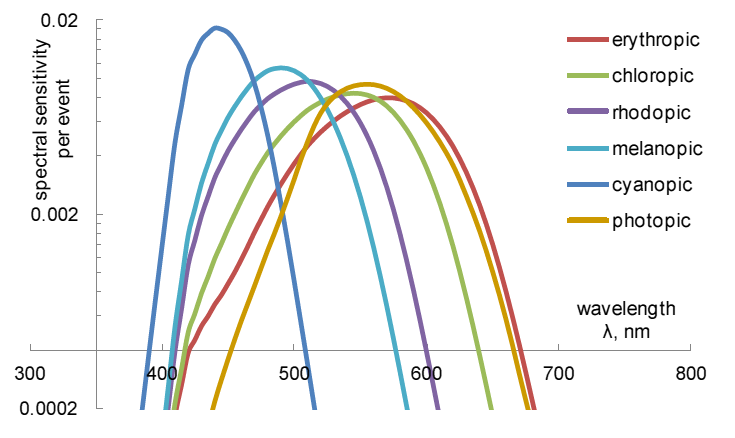
\includegraphics[max width=\textwidth, center]{figs/LitRev/ciemel.png}
\caption{Reproduced from \gls{CIE} TN 003:2015 \citep{cie_cie_2015-1}. \textit{``Spectral sensitivity curves of the five human photopigments to irradiance at the outer surface of the eye of the standard observer and photopic spectral efficiency, normalized to equal area.''}}
\label{fig:specsens}
\end{figure}

Exogenously expressed mouse melanopsin has been shown to be tristable \citep{emanuel_melanopsin_2015,matsuyama_photochemical_2012-1}, that is: existing in one of three possible states. A photon interaction converts melanopsin in one of these states to another, with two of the states being electrically silent (not providing a signal) and one being signal-producing. Notably, these different states have slightly different spectral sensitivities, and thus exposure to specific wavelengths biases the population distribution in different ways, as shown in Figure \ref{fig:melssf}.

\begin{figure}[htbp]
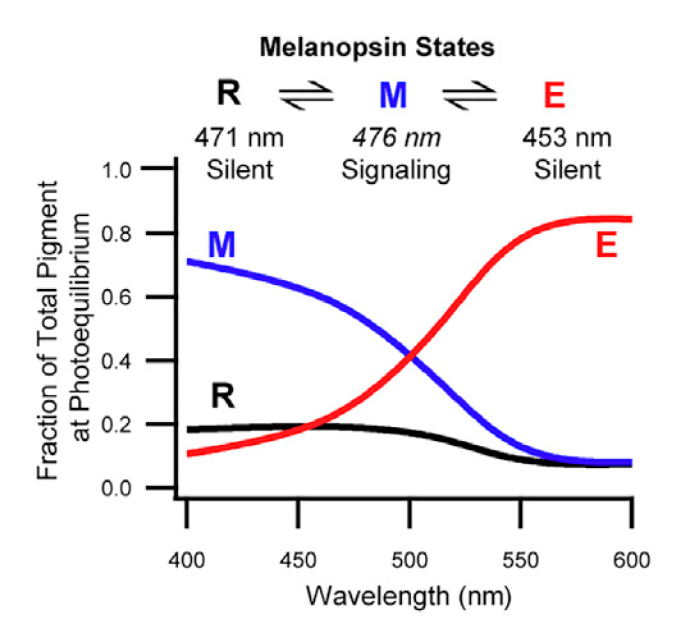
\includegraphics[max width=\textwidth, center]{figs/LitRev/melstates.png}
\caption{Reproduced from \citet{do_melanopsin_2019} (Fig 5D in original source). \textit{``[M]ouse melanopsin is understood to have three states (R, M, and E). The peak spectral sensitivities of R and E are determined from the electrophysiological responses of M1s. Spectrophotometric measurements of purified melanopsin yielded similar values (467 and 446 nm, respectively) and gave information for M (476 nm; [\citet{matsuyama_photochemical_2012-1}]). Bottom, the distribution of melanopsin states as a function of wavelength, estimated from a model based on values from purified melanopsin.''}}
\label{fig:melssf}
\end{figure}

Human melanopsin appears to be bistable (of two states), and there is uncertainty regarding whether this bistability has physiological consequences \citep{cie_cie_2015-1,mure_melanopsin_2009,rollag_does_2008,wada_color_2018,mure_melanopsin-dependent_2007,mawad_absence_2008,koyanagi_cephalochordate_2005,emanuel_melanopsin_2015}. It has been shown in other organisms that colour opponency from a single opsin is possible \citep{wada_color_2018}.

\Glspl{ipRGC} form a sparse mesh across the retina, each covering roughly 10$^{\circ}$ of visual angle \citep{ecker_melanopsin-expressing_2010}; discounting input from other cell types, they operate at a much lower resolution than as would be required for spatial vision of the type we are accustomed to. 

They also operate much more slowly than other cell types, taking several seconds to respond, but are able to sustain a response in contrast to other retinal cell types which are able to respond quickly but only for short periods (See Figure \ref{fig:melspeed} and \citet[p.210]{do_melanopsin_2019} for a summary).

\begin{figure}[htbp]
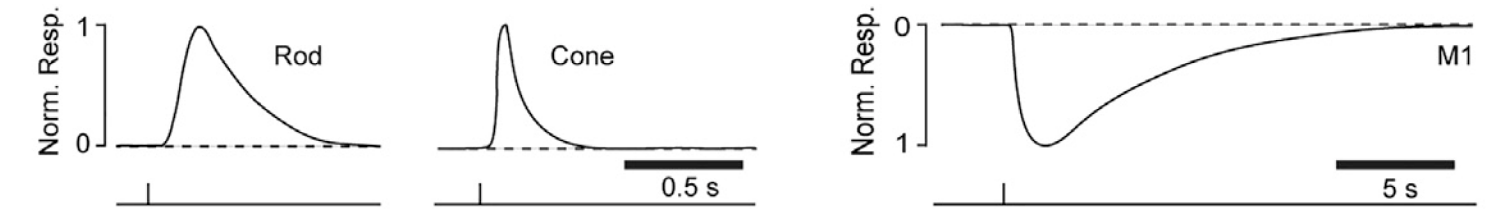
\includegraphics[max width=\textwidth, center]{figs/LitRev/melspeed.png}
\caption{Reproduced from \citet{do_melanopsin_2019} (Fig 5B in original source). \textit{``Dim-flash responses of outer photoreceptors and M1s (normalized photocurrent, having the same waveform as the single-photon response). Note the 10-fold
longer time base for the M1. The dashed line indicates the baseline current and the timing of the flash is shown below the curves, which are traced from
electrophysiological recordings (\citet{emanuel_biophysical_2017,field_nonlinear_2002,nikonov_physiological_2006}).''}}
\label{fig:melspeed}
\end{figure}

\Glspl{ipRGC} vary greatly in the range of light intensities that they are sensitive, are unimodal (stop responding above a certain threshold), and as a population their sensitivity spans a large range of lights levels \citep{do_melanopsin_2019}. It has been proposed that these properties \glspl{ipRGC} would allow an observer to efficiently sense a level of absolute irradiance \citep{brown_melanopsin_2010,milner_population_2017} (restricted to the wavelengths which ipRGCs and their inputs are sensitive to). 

\subsection{Synaptic Input}

In addition to their intrinsic photosensitivity, \glspl{ipRGC} exhibit extrinsic photosensitivity, taking inputs from rod and cone pathways in a similar fashion to regular \glspl{RGC}. Synaptic input is provided by amacrine and bipolar cells (See \citet{belenky_melanopsin_2003} and Figures \ref{fig:lucas} and \ref{fig:do}). 

\begin{figure}[htbp]
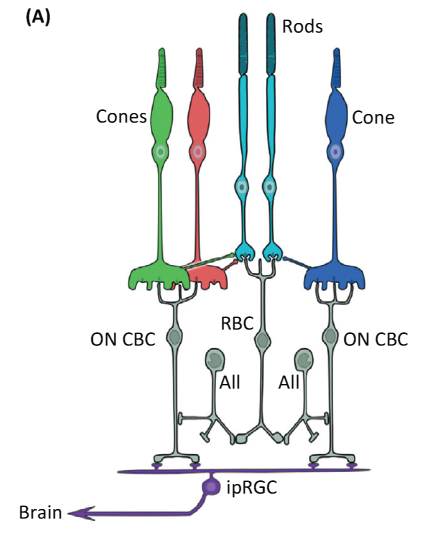
\includegraphics[max width=\textwidth, center]{figs/LitRev/lucas.png}
\caption{Reproduced from \citet{lucas_measuring_2014} (Figure 1A in origial source). \textit{``Schematic of the relevant retinal circuitry in humans. Non-image-forming responses originate in the retina and have been attributed to a particular class of retinal ganglion cell (ipRGC). ipRGCs are directly photosensitive owing to expression of melanopsin, which allows them to respond to light even when isolated from the rest of the retina. In situ they are connected to the outer retinal rod and cone photoreceptors via the conventional retinal circuitry. The details of their intraretinal connections are not completely understood and probably vary between different subtypes. Shown here are major connections with on cone bipolar cells (on CBCs) connecting them to cone and, via amacrine cells (AII) and rod bipolar cells (RBC), rod photoreceptors. As a consequence, the firing pattern of ipRGCs can be influenced by both intrinsic melanopsin photoreception and extrinsic signals originating in rods and each of the spectrally distinct cone classes (shown in red, green, and blue).''}}
\label{fig:lucas}
\end{figure}

\begin{figure}[htbp]
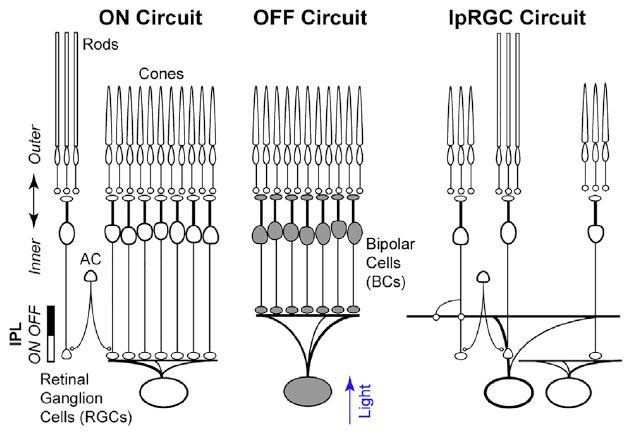
\includegraphics[max width=\textwidth, center]{figs/LitRev/do.png}
\caption{Reproduced from \citet{do_melanopsin_2019} (Fig 1A in original source). \textit{``A highly simplified schematic of the retina in cross-section, oriented with the inner aspect (nearer the center of the eye) down. The outer photoreceptors (i.e., rods/cones) drive bipolar cells (BCs). In the inner plexiform layer (IPL), BCs synapse with retinal ganglion cells (RGCs). Left: ON circuitry. Rods (top) drive rod BCs, whose signals pass through amacrine cells (ACs) to cone BCs. In the inner IPL, ON cone BCs convey signals to ON RGCs. ON RGCs show greater depolarization when light intensity increases. Center, OFF circuitry. In the outer IPL, OFF cone BCs provide synaptic input to OFF RGCs. OFF RGCs show greater depolarization when light intensity decreases. Right: a sample of circuits for outer- and inner-stratifying ipRGCs, which are both ON. ON cone BCs make ectopic synapses with the former and conventional synapses with the latter. Rod pathways also drive ipRGCs. IpRGCs make chemical and electrical synapses with ACs (not shown).''}}
\label{fig:do}
\end{figure}

Inputs evoke ON responses, despite originating from both the ON and OFF layers of the inner plexiform layer (see Figure \ref{fig:do}). \citet{graham_melanopsin-expressing_2016} describe the processes which allow this to occur: 

\begin{itquote}{}
ON bipolar cells use two unconventional strategies to release glutamate onto the dendrites of SCN-projecting mouse ipRGCs in the “OFF” sublamina. Some ON bipolar cells’ axons extend lateral protrusions that contain synaptic vesicles [...], whereas others possess en passant (in passing) synaptic vesicles within their axonal shafts [\citet{dumitrescu_ectopic_2009}]. Distally stratifying ipRGCs are also present in rabbit, marmoset and macaque retinas, and they likewise receive unconventional ON bipolar input in the “OFF” sublamina [...] [\citet{hoshi_inputs_2009}, \citet{grunert_bipolar_2011}].
\end{itquote}

Signals from rods and cones retain their traditional time courses; \glspl{ipRGC} are not inherently sluggish, rather the melanopic inputs to \glspl{ipRGC} are. This can be seen in Figure \ref{fig:wong}, where standard outputs of an \gls{ipRGC} are shown on the left, and outputs with rod/cone driven synaptic inputs blocked are shown on the right. The response is shown to be relatively instantaneous for the cell with intact inputs, but lagging by several seconds for the cell relying on melanoptic activation alone.

\begin{figure}[htbp]
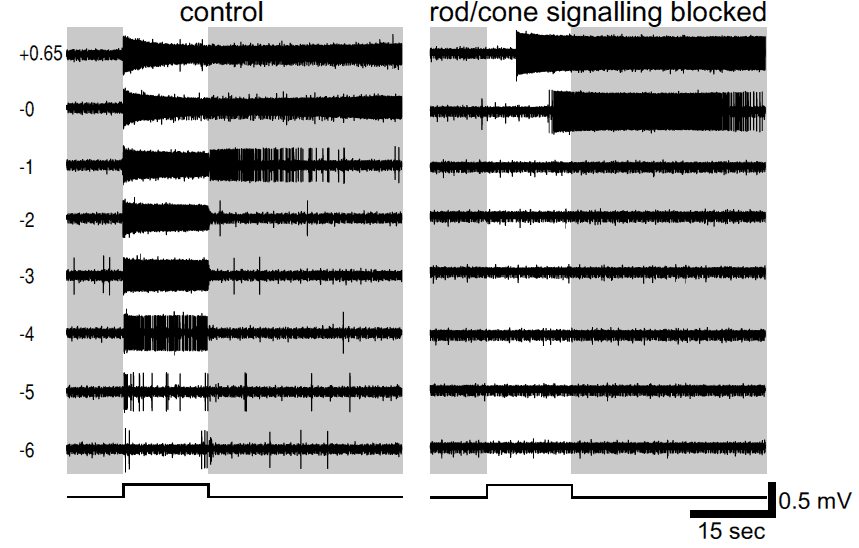
\includegraphics[max width=\textwidth, center]{figs/LitRev/wong.png}
\caption{Reproduced from \citet{wong_synaptic_2007} (Fig 4 in original source). \textit{``Multi-electrode array (MEA) recordings of synaptically mediated light responses in ipRGCs. Extracellular recordings comparing spike responses of an ipRGC to light of various intensities with rod/cone-driven synaptic inputs left intact (left) or blocked (right). Log stimulus attenuation is indicated to the left. Note that all responses to weaker stimuli (-2 log attenuation and dimmer) and short-latency responses to brighter ones (-1 to +0.65 log I) were dependent on synaptic transmission, presumably because they reflect rod and/or cone influence on the recorded cell. Note also that intensities sufficient to recruit the intrinsic response (-0 and +0.65 log I; right) evoke responses with substantial poststimulus persistence, a well-established feature of melanopsin-dependent light responses.''}}
\label{fig:wong}
\end{figure}

There also evidence for \glspl{ipRGC} having intraretinal retrograde synaptic output (\citet{zhang_intraretinal_2008,zhang_melanopsin_2012}, summarised by \citet{graham_melanopsin-expressing_2016}), via a subpopulation of dopaminergic amacrine cells. This type of signalling could provide a feedback loop which modifies signals before they have left the retina.

\subsection{Projection}

\glspl{ipRGC} have been shown to innervate `dozens of brain areas' \citep{do_melanopsin_2019}, with M1s principally innervating \gls{NIF} areas, but with some activation of areas traditionally thought of as image-forming. There appear to be meaningful differences between the different sub-types of \gls{ipRGC} in this respect, with different sub-types (denoted M1-6, distinguished by their retinal morphology) showing distinct activation pathways. 

A summary of these projections is shown in Figure \ref{fig:projection}. From this figure it can be seen that there are still many potential projections which have not been investigated (``Each blue dot indicates the approximate density of innervation by its size, a white dot indicates undetectable innervation, and lack of a dot indicates an absence of information.''). However, it can clearly be seen that outputs are extensive and varied.

\begin{figure}[htbp]
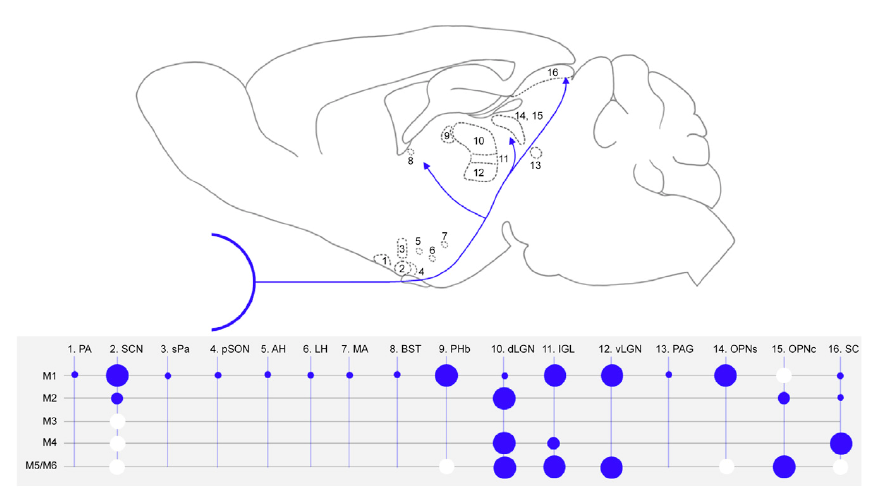
\includegraphics[max width=\textwidth, center]{figs/LitRev/projection.png}
\caption{Reproduced from \citet{do_melanopsin_2019} (Fig 3 in original source). \textit{``Major Brain Targets of Mouse IpRGCs. A sample of ipRGC brain targets is depicted in a quasi-sagittal schematic of the mouse brain. Below is a plot of innervation densities across ipRGC types, drawn after Berson and colleagues (\citet{quattrochi_m6_2019}) and incorporating additional information (\citet{ecker_melanopsin-expressing_2010}; \citet{hattar_central_2006}; \citet{huang_visual_2019}; \citet{morin_retinofugal_2014}; \citet{zhao_photoresponse_2014}). Each blue dot indicates the approximate density of innervation by its size, a white dot indicates undetectable innervation, and lack of a dot indicates an absence of information. M5s and M6s are pooled because their projections were examined together for technical reasons. AH, anterior hypothalamus; BST, bed nucleus of the stria terminalis; dLGN, dorsal lateral geniculate nucleus; IGL, intergeniculate leaflet; LH, lateral hypothalamus; MA, medial amygdala; OPN, olivary pretectal nucleus (with shell, s, and core, c, regions); PA, preoptic area, which includes the VLPO (ventrolateral preoptic area); PAG, periaqueductal gray; PHb, perihabenular zone; pSON, peri-supraoptic nucleus; SC, superior colliculus; SCN, suprachiasmatic nucleus; sPa, subparaventricular zone; and vLGN, ventral lateral geniculate nucleus.''}}
\label{fig:projection}
\end{figure}

\subsection{The roles of ipRGCs beyond circadian entrainment}
\label{sec:ipRGCbeyond}

In recent years there has been a number of publications examining the role of melanopsin outside of \gls{NIF} vision, challenging some of the assumptions about the roles of the signals originating from \glspl{ipRGC}.

A number of studies have found that the signals from ipRGCs are capable of encoding spatial structure \citep{ecker_melanopsin-expressing_2010, mouland_responses_2017, allen_melanopsin_2017, allen_form_2019, zhao_photoresponse_2014}\footnote{For commentary see \citet{spitschan_vision_2017} and \citet{sonoda_re-evaluating_2016}.}, and others have probed the influence upon brightness perception \citep{zele_cone_2018,brown_melanopsin-based_2012}.

Additionally, several researchers have investigated whether \glspl{ipRGC} may play a role in chromatic vision \citep{cao_evidence_2018, spitschan_human_2017-1,zele_melanopsin_2018,horiguchi_human_2013,vincent_adaptation_2019,vincent_adaptation_2019-1}, using the silent substitution paradigm \citep{estevez_silent_1982,spitschan_method_2018}\footnote{Though see \citet{kamar_silent-substitution_2019}.}. These studies are summarised below.

\textbf{\citet{spitschan_human_2017-1}} found an fMRI response in primary visual cortex for each of four participants, in contradiction to an earlier study by the same group \citep{spitschan_human_2016}\footnote{``we now regard our prior study as not fully resolving the possibility that rapid modulation of the ipRGCs drives a cortical response'' \citep{spitschan_human_2017-1}}. Participants reported a visual percept which was ``unpleasant, blurry, minimal brightening that quickly faded''. There was also some evidence of a chromatic percept: ``Many of the subjects described the melanopsin stimulus pulse as being colored. This was typically a yellow–orange appearance, although three subjects reported a greenish percept''.


\textbf{\citet{cao_evidence_2018}} found that ``changing melanopsin activation levels shifts the equilibrium point in the chromatic pathways'', though curiously the effect was only present for the L/(L+M) pathway. The key figure from this study is reproduced in Figure \ref{fig:cao}. 

The authors conclude that melanopsin activation affects the parvocellular pathway to the extent that \gls{ipRGC} activation could be thought of as ``additive to the M-cone signal opposing the L-cone signal in the PC pathway [i.e., L - (M + I)] (where ``I'' for melanopsin activation in ipRGCs) to signal greenness and/or blueness''. 

The authors note that this corresponds to an earlier result from one of the same authors \citep{barrionuevo_contributions_2014} where such a contribution set was proposed. However, the earlier result includes rod contributions, and the specific pathway which they must be referring to is only the 5th component accounting for $<0.01\%$ of the variance in the signals under examination. Meanwhile, no evidence is found for the 2nd component from that same analysis (labelled as konioncellular, representing $1.56\%$ of variance), which they also proposed would have a considerable melanopic contribution contribution. They neglect to mention this in the later paper.

\begin{figure}[htbp]
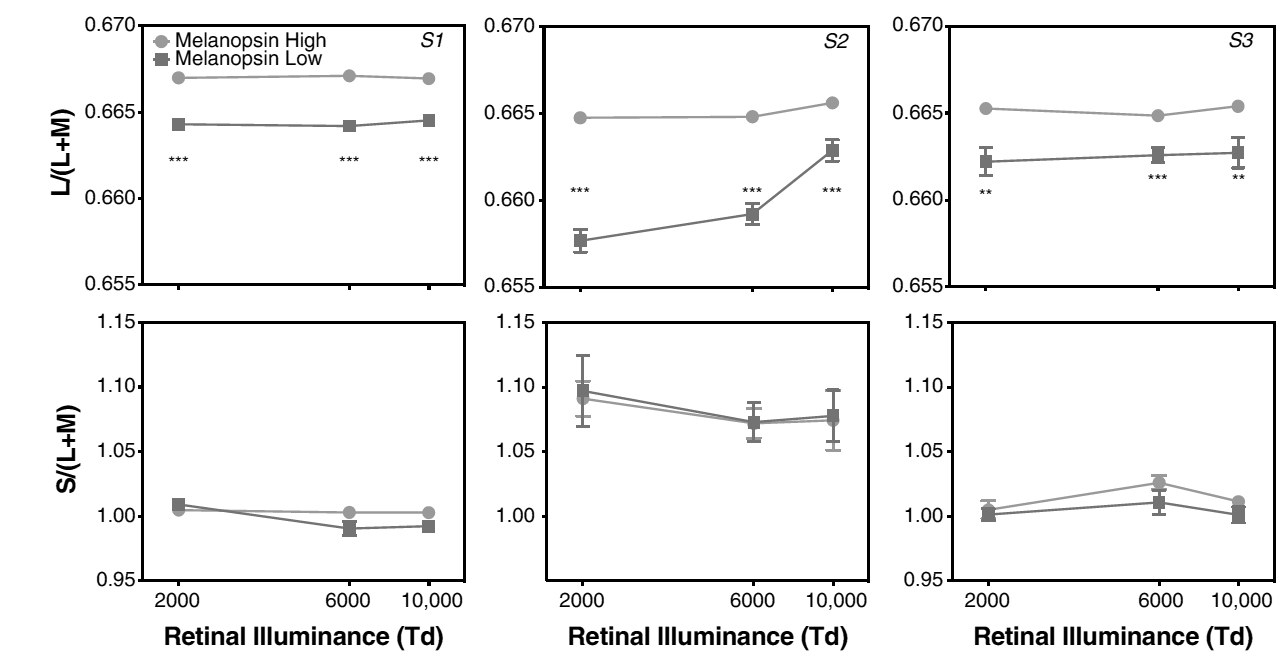
\includegraphics[max width=\textwidth, center]{figs/LitRev/cao.png}
\caption{Reproduced from \citet{cao_evidence_2018} (Figure 1 in original source). \textit{``Unique white $l$ (top) and $s$ (bottom) values (mean $\pm$ sem)
as a function of retinal illuminance for three observers. **$p < 0.01$;
***$p < 0.001$ from t-tests.''}}
\label{fig:cao}
\end{figure}

\textbf{\citet{zele_melanopsin_2018}} found evidence that ``putative melanopsin-mediated image-forming vision corresponds to an opponent S-OFF L+M-ON response property, with an average temporal resolution up to approximately 5 Hz, and $>$10x higher thresholds than red-green colour vision''. The key figure from this study is reproduced in Figure \ref{fig:zele}. This figure shows the perceptual matches to melanopic contrasts in terms of equivalent cone contrasts, for four observers, under three different conditions. For each observer, and for each condition, it can be seen that a melanopic contrast can be matched by an L+M increment and a S/(L+M) decrement.

\begin{figure}[htbp]
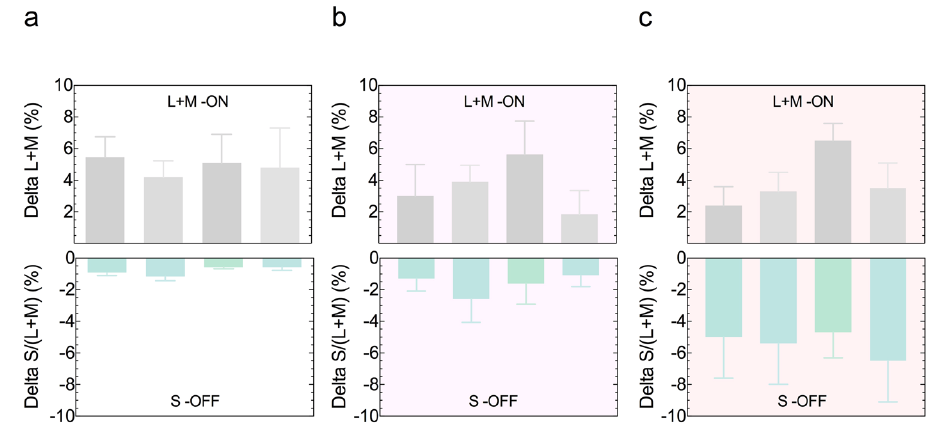
\includegraphics[max width=\textwidth, center]{figs/LitRev/zele.png}
\caption{Reproduced from \citet{zele_melanopsin_2018}. \textit{``Melanopsin photoreception is analogous to an increment in cone luminance [L + M] and a decrement in S-cone excitation [S/(L + M)] with white (a), yellowish-pink (b) and orange adapting stimulus fields (c). [...] Data in each panel are for four participants (mean $\pm$ SEM) measured at 2000 photopic Td.''}}
\label{fig:zele}
\end{figure}

This appears to be a perfect contradiction to the results of \citet{cao_evidence_2018}: \citet{cao_evidence_2018} found a parvocellular response and no koniocellular response whilst \citet{zele_melanopsin_2018} found a koniocellular response\footnote{Albeit inverted: S-OFF L+M-ON, rather than the traditional S-ON L+M-OFF \citep{hendry_koniocellular_2000}.} and no parvocellular response\footnote{Though the matching values for this pathway aren't actually reported. One assumes they did not exhibit a trend and/or fell below some meaningful threshold.}. However, attention should be paid to the distinctions in experimental goals and procedures. \citet{cao_evidence_2018} probe the long term adaptive effects of differing levels of melanopic activation upon white settings, whereas \citet{zele_melanopsin_2019} probe the equivalent appearance of melanopsin in terms of cone-based percepts. It is possible that this distinction is the root of the inconsistency.

\textbf{\citet{horiguchi_human_2013}} found that ``[i]n the periphery, at high photopic levels, human sensitivity is not accurately explained by absorptions in only three types of cone photopigments [and requires a fourth]''. This work focuses on discrimination thresholds rather than attempting to understand a direct perceptual correlate to melanopic stimulation. They conclude that ``[t]he most likely hypothesis is that in healthy human subjects melanopsin absorptions influence visibility.''

Very recent results from \textbf{\citet{vincent_adaptation_2019,vincent_adaptation_2019-1}} report that, contrary to expectations (based on the work of \citet{allen_melanopsin-driven_2014}), ``sensitivity to flicker directed at the cones was not altered by adaptation to a steady field of substantially higher melanopic content''. This appears to rule out the hypothesis that melanopsin activation alters gain (aka adaptation) at an early retinal level for cone-based signals.

Though all the above results are exciting, there are a number of methodological and theoretical areas which require development. The standard methodology used in these experiments is that of `silent substitution' \citep{estevez_silent_1982,kamar_silent-substitution_2019,spitschan_method_2018} where careful tuning of the spectrum is used (see the topic of `metameric blacks' \citep{vienot_verriest_2014,cohen_metameric_1982,vienot_domain_2012,vienot_dimensionality_2015}) to generate signals which are only visible to the chosen receptor-type in theory, in this case melanopsin-expressing \glspl{ipRGC}. 

However, due to variability in observer spectral sensitivities, and limits on the level of stimulus control, it is likely that there will be a small amount of unintended stimulation of non-target cell groups. \citet{spitschan_selective_2015} refer to this as `splatter' (``the expected amount of contrast on nominally silenced photoreceptor classes for a given modulation around a given background''). A suggested control condition is to generate contrast for the nominally silenced cell groups at the level predicted from modelling.

A further concern is that horizontal cell feedback, or other intraretinal retrograde signalling, could result in nominally silenced cone populations still producing an output \citep{kamar_silent-substitution_2019}.

\subsection{Value for colour constancy}

\emph{In this section I shall outline the reasoning which suggests to me that there might be value in a melanopic input for attaining colour constancy.}

Existing colour constancy algorithms fundamentally rely on the ability of cone-receptor-based signals to calibrate cone-receptor-based signals. In this context, by \emph{calibrate} I mean  \emph{modify a raw signal in order to exclude unwanted signal, in order to improve the accuracy (and possibly also precision) of target signal measurement} where the \emph{unwanted signal} would be variation in illumination, and the target signal would be either the \gls{SRF} of a surface or some other identifier of the surface.

This general framework suffers from what I refer to as the issue of circularity in self-calibration\footnote{I suspect that this issue has been discussed in other fields but I have been unable to find such discussion as of yet.}. Generally calibration is performed by characterising a sensor through measurement of an object where the ground truth is known (and/or a measurement from a trusted secondary sensor has been made of this object), and adjusting the properties of the sensor (either at the measurement stage or by implementing a post-processing stage) such that a measurement of the known object results in the expected values. In the case outlined above (cone-receptor-based signals calibrating cone-receptor-based signals), there is no ground truth object, and no secondary sensor, and thus calibration in the traditional sense fundamentally cannot be performed.

If only relative signals are of importance (as opposed to absolute value measurements), then an uncalibrated system might achieve satisfactory stability through the use of measurements taken over time or over space from a single sensor.

A melanopic signal could represent a secondary signal, and the properties of \glspl{ipRGC} seem to make them well-suited for making measurements where the ambient illumination is preferentially detected over transient \glspl{SRF}. Particular properties will be discussed below.

If one's goal was to design a sensor which measured the ambient illumination upon a scene (and was only minimally perturbed by surface reflectances) it might be wise to limit both the spatial and temporal resolution relative to sensors which may be best for measuring surfaces, since the lighting on a scene generally operates at spatial and temporal frequencies which are both lower than surface variation within a scene, particularly when the scene is not viewed from a static position but from a constantly changing vantage (such as is the case with human vision, where the observer is moving body, face direction, and gaze direction regularly). It would also be ideal if the secondary sensor was not strongly adaptive, as this would allow for a more concrete relationship between stimuli and response. \Glspl{ipRGC} exhibit all of the above properties.

There are multiple sites at which a melanopsin-based calibration could occur. The synaptic connections to \glspl{ipRGC} from rods and cones could allow a melanopsin-dependent transform to be performed at the \gls{RGC} stage before signals are output. Alternatively, the intraretinal outputs from \glspl{ipRGC} could allow for modification of signals before reception by traditional \glspl{RGC}. Finally, calibration could occur at any higher post-retinal location assuming that melanopic and cone-based signals could be reconstructed at that point.





\clearpage




\subsection{Peripheral vision}


\section{Museum Lighting}

\bigskip

\begin{itquote}{}
Museums and art galleries collect, preserve, and display natural artifacts and/or examples of human achievement and analyze their impact on the world and the universe around us. Effective exhibit lighting must balance exhibition and conservation needs and enrich the museum experience.
\end{itquote}

\begin{flushright}IES RP-30-96 Museum and Art Gallery Lighting: \\A Recommended Practice \citep{ies_ies_1996}\end{flushright}

\bigskip

Lighting in museums is required to satisfy multiple criteria; perhaps the least contestable requirement being that the lighting illuminate objects such that they are suitably visible to museum visitors. Also of utmost importance in most museum settings is that the lighting does not have an unreasonably damaging effect upon the objects or environment, be this through direct photodegradation or as a result of heat transfer. Further to these requirements, an increased or optimal visual quality is generally desirable, although what this represents or how to achieve it is generally ambiguous.

In sweeping terms, all electromagnetic radiation (visible and non-visible) damages objects, and more radiation damages objects proportionally moreso. Thus the question becomes: \emph{how little light can we use to illuminate objects such that they're visible to the extent required?} The inverse form, sometimes used on the assumption that more light always represents an increase in observer satisfaction/pleasure is: \emph{`how much light can we use so that only $x$ damage occurs over $y$ time'}. 

Industry guidance documents provide advice on how to manage lighting to best address the above requirements and many other additional specific requirements through the recommendation of procedure and provision of target figures for quantitative variables. \Gls{UV} radiation, being of no visual benefit but having potential to harm, is now excluded from gallery spaces as an industry standard. %KC: citation required

%KC: I would add a summarising sentence here e.g. "This section discusses existing literature covering the various factors that need to be considered when choosing a museum light source, specifically those that relate to its SPD.  These include the likelihood of damage and the visitor experience.  A discussion of existing museum guidance on these topics is also provided.

\subsection{Damage functions} \label{sec:DamageIndex}

%KC: Can you link this to the ipRGCs?  Overall, this shows that in terms of material damage, the wavelengths to avoid are the low ones and that light sources which have high intensities at the peak sensitivity of melanopsin could be considered as not particularly hazardous for museums.

\textit{The key reference on this subject is \gls{CIE} 157:2004 \citep{cie_cie_2004}, and valuable talks on the subject were given at the recent Museum Lighting Symposium \& Workshops \citep{pokorska_book_2017} (which the author helped to organise), and have been made freely available online\footnote{See in particular the talks by David Saunders (\url{https://www.youtube.com/watch?v=H4d0qH0IBcI&t}) and Stefan Michalski (\url{https://www.youtube.com/watch?v=XUY9biLQqlw}).}}.

\bigskip

In heritage science `damage functions' are ``functions of unacceptable change, dependent on agents of change'' \citep{strlic_damage_2013}. The goal of damage functions in heritage lighting engineering is to give a quantitative means by which to predict the amount of damage caused to a prototypical object by a given light source, and to assist in limiting such damage. They generally follow the logic that radiation of lower wavelength is likely to cause more damage to objects.

\citet{harrison_report_1953} is generally acknowledged as the first to suggest such a function, but he himself acknowledges that it had ``long been established that the shorter the wavelength (visible yellow, green, blue, violet and invisible UV being progressively shorter) the more photochemically potent will be such radiant energy, provided such energy is actually absorbed''. \citet[p.9]{harrison_report_1953} defined the `radiation hazard associated with a light source' as:

\begin{equation}
    \sum_{0}^{\infty} \mathrm{H}_{\lambda} \mathrm{D}_{\lambda} \Delta \lambda / \sum_{0}^{\infty} \mathrm{H}_{\lambda} \overline{\mathrm{y}}_{\lambda} \Delta \lambda
    \label{eq:Harrison}
\end{equation}

where $\mathrm{H}_{\lambda}$ is the spectral irradiance, $\mathrm{D}_{\lambda}$ is the `Relative Damage Factor' (which is extrapolated from the data collected shortly prior to Harrison's own report by the National Bureau of Standards \citep{national_bureau_of_standards_preservation_1951}, and shown in Figure \ref{fig:Harrison}), and $\overline{\mathrm{y}}_{\lambda}$ is the \gls{CIE} 1924 photopic $V_{\lambda}$ luminosity function. The resulting value would describe the amount of damage expected from a light source, normalised by its luminance.

\begin{figure}[htbp]
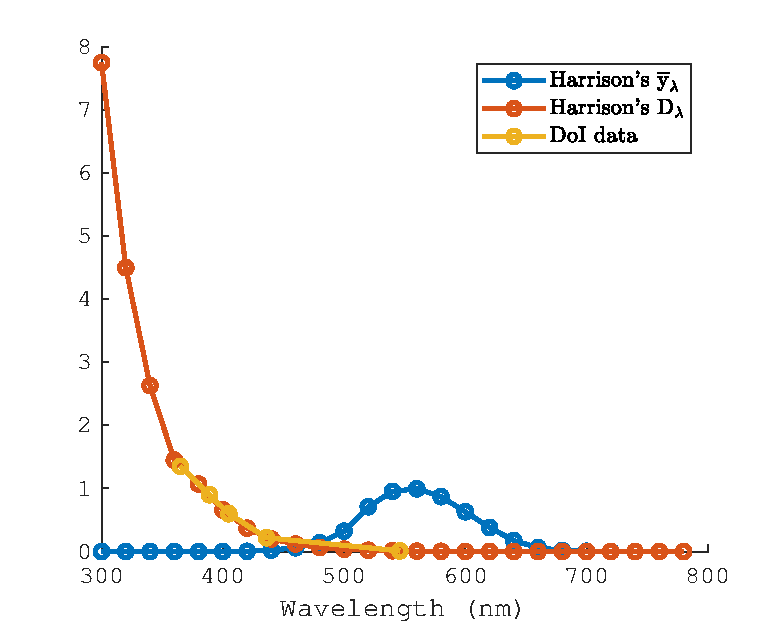
\includegraphics[max width=\textwidth]{figs/LitRev/HarrisonAndDoI.pdf}
\caption{Harrison's \citep{harrison_report_1953} damage function ($\mathrm{D}_{\lambda}$), and luminous efficacy ($\overline{\mathrm{y}}_{\lambda}$), alongside the Declaration of Independence data \citep{national_bureau_of_standards_preservation_1951} from which it was extrapolated (re-normalised to match scale).}
\label{fig:Harrison}
\end{figure}

\begin{figure}[htbp]
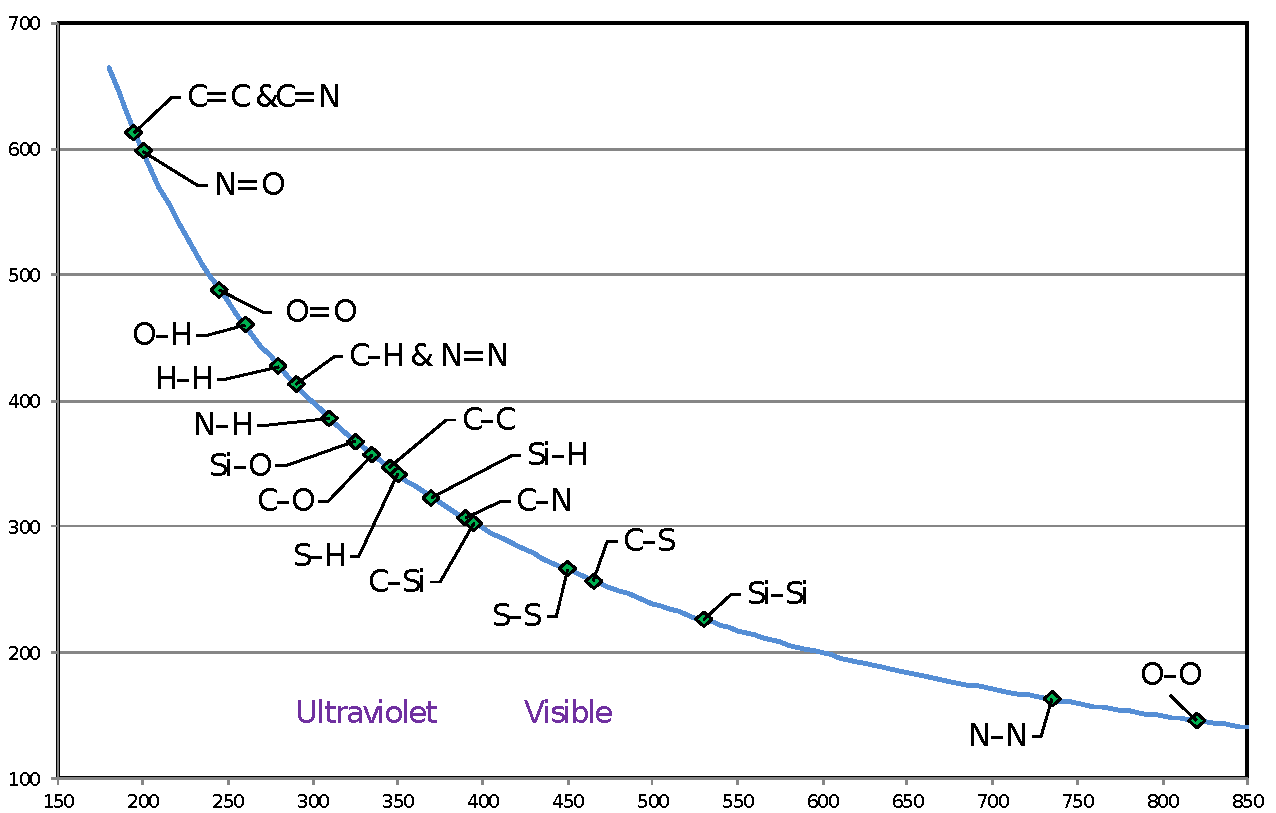
\includegraphics[max width=\textwidth]{figs/LitRev/Saunders.pdf}
\caption{Graph courtesy of David Saunders, presented at the Museum Lighting Symposium \& Workshops \citep[p.61]{pokorska_book_2017} showing the relationship between wavelength and the bonds which can be broken in various molecules, with `Wavelength (nm)' on the abscissa and `Bond energy (kJ/mol)' on the ordinate.}
\label{fig:Saunders}
\end{figure}

There has been extended scepticism about the utility of damage functions in general, with the argument being that no one damage function could represent the vast range and complexities of real materials. \citet[p. 178]{thomson_museum_1978} wrote that ``for more fugitive materials \dots the figure for visible radiation would be higher. On the other hand \dots the fastest dyes are probably affected only by UV. Thus it can be seen that no single figure can be given for damage versus wavelength''.

Criticism was aimed at this specific damage function due to its derivation from such a small and minimally representative dataset - Harrison's data was `extended' from the 5 datapoints measured by the National Bureau of Standards \citep{national_bureau_of_standards_preservation_1951} in their investigations of how to best care for the Declaration of Independence\footnote{It is a curiosity that these minimal figures would not in fact have been much use to those planning the care for the declaration, since in the report it is noted that ``The deterioration of animal parchment is not as rapid as that of the low-grade paper for which the damage factors were determined'' \citep{national_bureau_of_standards_preservation_1951}, and the Declaration of Independence is written on animal parchment.}, and was derived from the study of `low-grade paper', which cannot to said to represent the average museum item\footnote{Though \emph{no} material truly can!}.

\gls{CIE} 157:2004 \citep{cie_cie_2004} notes that whilst Harrison's proposal failed to gain acceptance as the procedure for comparing the damage potential of different types of light sources, it did convince people of the ills of \gls{UV}, with the result that daylight was subsequently eliminated from many galleries.

Following \citet{cuttle_lighting_1988}, who noted that Harrison's damage function could be well fit by an inverted logarithmic function, with parameters controlling the slope and normalisation point of the function, \gls{CIE} 157:2004 provided the following equation:

\begin{equation}
    s(\lambda)_{\mathrm{dm,rel}}=\exp [-b(\lambda-n)]
    \label{eq:damfac}
\end{equation}

where differing values of $b$ for 5 categories of item are provided (Table \ref{tab:b}), $n$ is the normalisation value (\gls{CIE} 157:2004 uses a value of 300), and the $s(\lambda)_{\mathrm{dm,rel}}$ function is the estimated action spectrum for each category. $s(\lambda)_{\mathrm{dm,rel}}$ would be substituted into Equation \ref{eq:Harrison} for $\mathrm{D}_{\lambda}$. \gls{CIE} 157:2004 also provides values of $H_{s,dm}$ which indicate the susceptibility of each group of materials to damage (where damage is considered as colour change%in $\Delta E_{\mathrm{ab}}^{\ast}$
).

\begin{table}[htbp]
\centering
\begin{tabular}{|c|l|l|l|}
\hline
Group & Samples & $H_{s,dm}$ (W h/m$^{2}$) & $b$ \\ \hline
a & Low-grade paper & 5 & 0.038 \\ \hline
b & Rag paper & 1200 & 0.0125 \\ \hline
c & Oil paints on canvas & 850 & 0.0115 \\ \hline
d & Textiles & 290 & 0.0100 \\ \hline
e & Water colours on rag paper & 175 & 0.0115 \\ \hline
\end{tabular}
\caption{Table reproduced from \gls{CIE} 157:2004 \citep{cie_cie_2004}, showing the values for $H_{s,dm}$ and $b$ for various categories. Note: the source for this data is not particularly clear; it is listed as `The Berlin researchers', which is assumed to follow the references: \citet{krochmann_beleuchtung_1988,cie_cie_1991,hilbert_zur_1991}; none of which I have been able to access.}
\label{tab:b}
\end{table}

The more general criticism that damage functions will never be able to represent all museum objects is a valid concern, and can be well illustrated with the following logic: museums own objects of many different colours, different colours arise from different reflectance properties, different reflectance properties mean different wavelengths are absorbed, and damage can only occur when radiation is absorbed. Thus it follows that one would expect two objects of different colours to have different damage functions. 

The classic study on how reflectance properties relate to damage is that of \citet{saunders_wavelength-dependent_1994}. They exposed a number of pigments to a range of wavelengths and measured the resulting damage.%KC: Can you give a bit more detail in this sentence?  Did Saunders and Kirby use a series of monochromatic light sources?  Did damage mean colour change here?
\citet{cuttle_control_1999} later replotted the data from this study (see Figure \ref{fig:Cuttle}), highlighting the apparent joint contributions of spectral reflectance and a general damage function to the individual damage functions. \gls{CIE} 157:2004 notes however that this correspondence is not perfect or easily modellable, and that ``a workable system for characterising action spectra for colorants, including pigments and dyes, remains an unattained goal''. Recent studied have added new data (see esp. \citet{villmann_wavelength_2018}), and it is hoped that a general understanding may at some point be reached.

\begin{figure}[htbp]
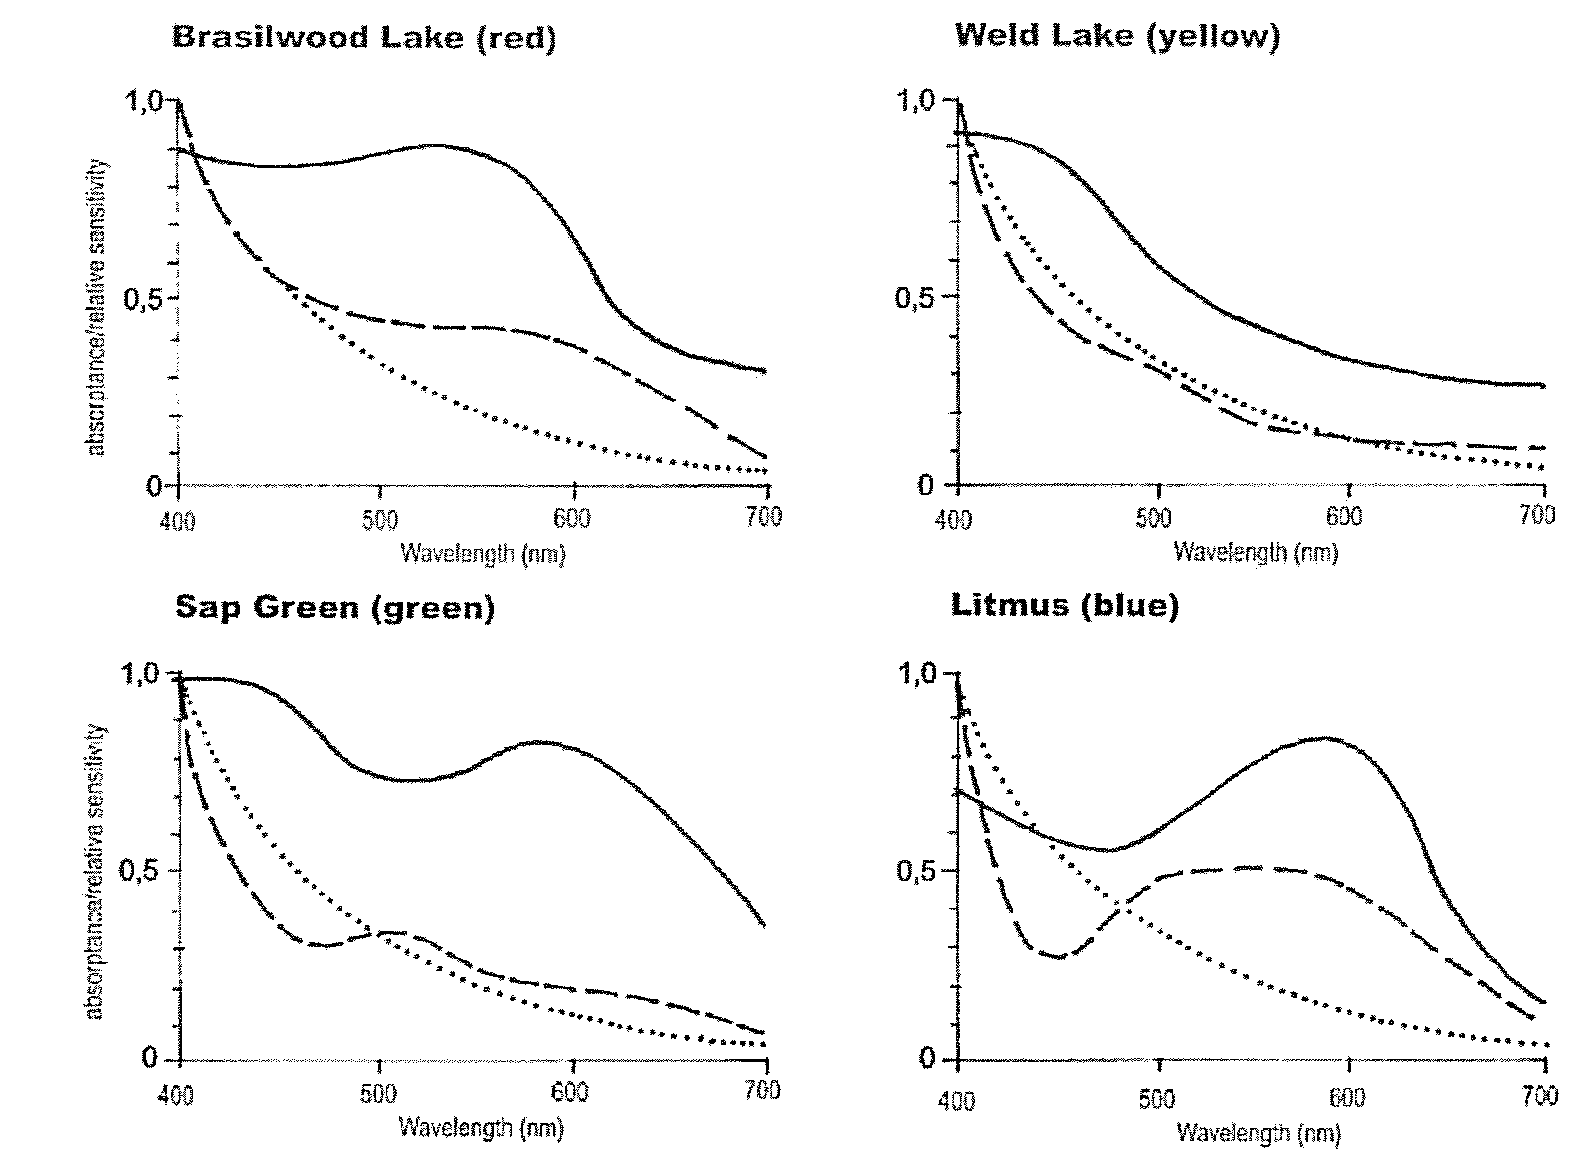
\includegraphics[max width=\textwidth]{figs/LitRev/Cuttle.png}
\caption{The original data for this figure is from \citet{saunders_wavelength-dependent_1994}, later re-plotted by \citet{cuttle_control_1999}, and reproduced (with the addition of the Berlin functions) by the authors of \gls{CIE} 157:2004 \citep{cie_cie_2004}. Caption from \gls{CIE} 157:2004: ``Spectral absorptance (solid line) and relative spectral responsivity (broken line) for artist's pigments \dots The dotted lines show relative spectral sensitivities normalised at 400nm based on the Berlin relative spectral responsivity function.''}
\label{fig:Cuttle}
\end{figure}

However, it is the opinion of this author that this argument is an exercise in artificial futility; whilst we may not be able to model the individual damage functions for every object in a museum, we may at least use one which has some bearing on the damage function, rather than the one which is implicitly used by museums currently - the \gls{CIE} 1924 luminosity function ($\overline{\mathrm{y}}_{\lambda}$ of Figure \ref{fig:Harrison}), which relates to the sensitivity of the human eye rather than any type of object. \citet{cuttle_lighting_1988} puts it well: ``The argument, then, is not whether we have a [damage] function which is correct, but whether we can improve usefully upon the likely reliability of the present system''. It is depressing that this was said in 1988 and yet little seems to have changed in practice (See Chapter \ref{chap:Interviews}).

In the case where specific objects/pigments of interest can be identified, and their individual damage functions calculated, there is valuable research to draw on regarding methods for optimising light sources to minimise damage, initiated by \citet{miller_evaluating_1993} and developed by many others \citep{durmus_optimising_2017,durmus_colour_2015,durmus_optimising_2015,durmus_object_2017,delgado_ramos_art_2009,delgado_lighting_2011,luna_selective_2015,cuttle_proposal_2000,vazquez_point_2017}. The fading of lead chromate in the paintings of Vincent van Gogh has captured public attention \citep{lewis_smith_will_2013} and has resulted in multiple studies looking at ways to optimise the illuminant for this one particular material \citep{lunz_can_2017,monico_degradation_2011}.

With modern computation, and access to datasets, it becomes relatively easy to calculate a value of \Gls{DI}. Figure \ref{fig:Houser} shows the results for such computations for 401 illuminants and light sources (as per Equation \ref{eq:Harrison}, using a damage factor computed as per Equation \ref{eq:damfac}, but further normalised such that Illuminant A has a reference value of 1)\footnote{The code to reproduce this is available from: \url{https://github.com/da5nsy/DamageIndex}}. It can be seen that whilst most illuminants cluster around 1 there is a broad range. It should be remembered that these illuminants would in no way indicate their relative damage index to an observer or a purchaser, unless one went to the effort to look up or measure the \gls{SPD} and compute the damage factor. A careful or careless choice in this respect could easily double or halve the amount of time an item could be exhibited before succumbing to terminal damage.

\begin{figure}[htbp]
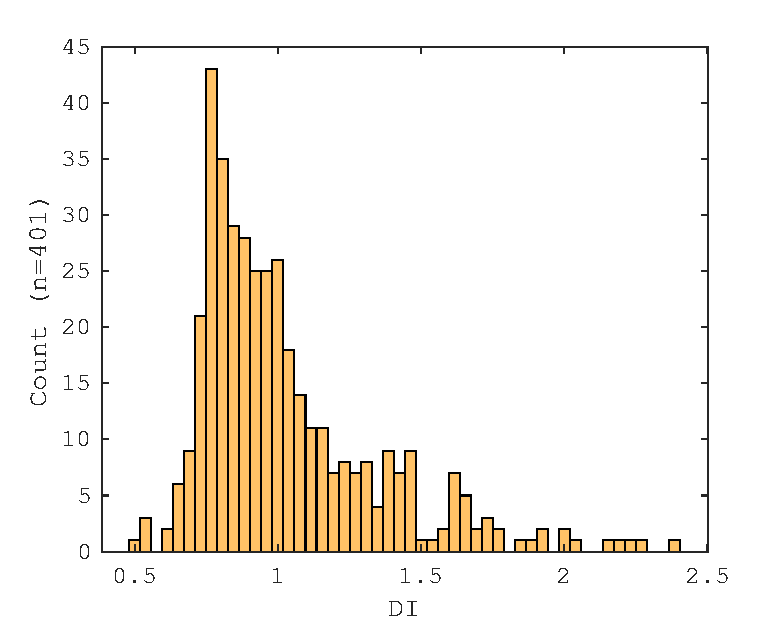
\includegraphics[max width=\textwidth]{figs/LitRev/DI.pdf}
\caption{The values of $DI$ for the 401 illuminants used by \citet{houser_review_2013}, available via \gls{PTB} as `spd\_houser', normalised such that \gls{CIE} Illuminant A receives a reference value of 1.}
\label{fig:Houser}
\end{figure}


\clearpage
\subsection{Visitor Requirements of Museum Lighting}

The visual requirements of museum visitors is likely to depend upon a large number of variables, both intrinsic and extrinsic to the visitor (e.g. intrinsic - age, cultural background, goals for the museum visit and extrinsic: luminance, lighting distribution, \gls{CCT}, \gls{CRI} and flicker properties of lighting). Some of these factors have been independently studied in a museum context, and for others it is likely that findings in other environments could generalise such that they could be used to inform decisions regarding museum lighting.

Traditionally, the principal manner in which museum professionals sought to limit damage was through setting a maximum luminance level. The implicit assumptions in this process are twofold; firstly: that damage will increase with increased luminance. This was a fairer assumption when tungsten was the only type of lighting technology, but as other lighting technologies with different \glspl{SPD} have been introduced this assumption has become less accurate (see Section \ref{sec:DamageIndex}: \nameref{sec:DamageIndex}). The second implicit assumption is that viewers will prefer higher luminance environments.

The classic study on this second assumption, performed in a mock-museum environment is that of \citet{loe_preferred_1982}. This research regards the display of oil and watercolour paintings specifically. In this study Loe et al. examined three variables: painting illuminance, light source (different technologies) and light distribution. Following the construction of a mock up gallery space, observers were asked to view paintings of various types under a range of illuminations, varying in `painting illuminance, light source and light distribution within the gallery space' and report upon semantic scales their perceptions. The results which informed the 200 lux recommendation stem from only the first variable, painting illuminance. Here it was found (as shown in Figure \ref{fig:Loe}) that for factors christened `discrimination' and `quality evaluation' (distilled from factor analysis of the original semantic data) there was `a steep rise in discrimination and quality assessment until and illuminance of approximately 200 lux is reached: above this illuminance the rate of increase in reduced.' This conclusion has had substantial impact in setting guidelines and future thinking was that a minimum of 200 lux was required to `give visual satisfaction', however it can be seen from Figure \ref{fig:Loe} that the data is sparse, noisy, dependent upon brand of illuminant and doesn't show a particularly strong effect of 200 lux in particular. Further, only a small number of different luminances were sampled, and it is quite possible that the results are at the mercy of several types of bias \citep{fotios_research_2009}. This figure was subsequently used in \citet{thomson_museum_1978}, which has informed a great deal of subsequent thinking on the topic.

\begin{figure}[htbp]
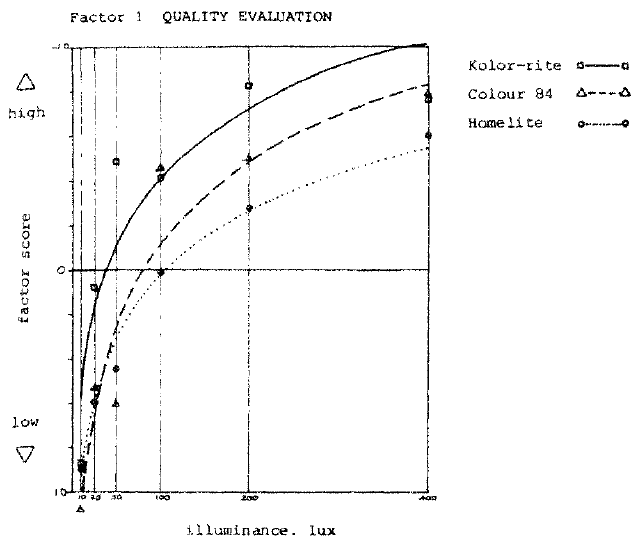
\includegraphics[max width=\textwidth]{figs/LitRev/Loe.png}
\caption{Illuminance vs a factor which is thought to indicate `quality', for three different brands of illuminant, reproduced from \citet{loe_preferred_1982}.}
\label{fig:Loe}
\end{figure}

There has been extensive research on the visitor requirements in terms of \gls{CCT} and \gls{CRI} and these shall be covered in separate sections.

In terms of a holistic approach to museum lighting research (considering more than a single or small number of isolated variables), there has been a great deal of work which deals with the visitor experience in a broad and cultured fashion from the lofty vantage of museum studies (such as \citet{falk_museum_2016} and \citet{shapiro_museum_1990}), but rarely do the physical practicalities such as lighting get a mention. 

The notable exception, where lighting as it relates to the visitor experience is considered, is the work of Kesner in the USA in the early nineteen-nineties \citep{kesner_museum_1993-1,kesner_museum_1993,kesner_exhibition_1992,kesner_current_1991,kesner_analysis_1997}.

Kesner's studies comprised self-reporting surveys, and concluded that colour accuracy was the highest requirement and that `richness' of colour was the lowest priority\footnote{A cautious interpretation of these results is advised, considering that there were high average scores for each category.}:

\begin{citequote}{kesner_museum_1993-1}
Artifact appearance, particularly clarity of artefact form and accuracy of artifact color, is the most important visitor need. Although visual impression, specifically acceptable gallery brightness and rich artefact color, is least important among the factors, it too rated highly important.
\end{citequote}

%more?

%Following the release of guidelines on the topic of \glspl{LED} in museums \citep{druzik_guidelines_2012}, a written survey of museum professionals who had requested these guidelines was performed, and the results reported by \citet{perrin_ssl_2014}. The respondents were predominately based in USA, with 30\% identifying as `international'. The survey was part of the USA government's `GATEWAY program'. Responding to the question `Please rank the following factors in your selection of lamps', joint first priorities are identified as `colour and spectral power distribution' and `damage potential'.

\subsection{Museum Lighting Specification Guidance Documents}

\textit{For a historical perspective on museum lighting guidance see \citet{druzik_museum_2007}.}

Five museum lighting guidance documents, thought to represent the most referred to documents in the field (informed by the interviews reported in Chapter \ref{chap:Interviews}), were reviewed. 

The purposes of this section:
\begin{enumerate}
\item To explore how museum professionals specify lighting, by understanding the tools and guidance which are available
\item To enquire as to what the guidance actually is, in terms of what subjects are covered and what the guidelines actually are
\item To question what these guidelines are based upon. How are the results of scientific study utilised in the production of these documents?
\end{enumerate}

Limiting the damage to museum objects by photodegradation is most often the responsibility of the preventive conservator within a museum, or the person holding a role which encompasses this role in the case of smaller institutions. It is therefore essential that the people in these roles have access to standardised and validated advice on how to approach the subject. Several overviews of the subject have been written and I shall aim to introduce the most prominent here, focusing on their aims, scope and differences/similarities. 

I shall operate a biased interest towards the recommendations regarding colour rendering, colour temperature, and illuminance level. Whilst the first two are the immediate area of study within this project, the third (luminance) is of interest for multiple reasons. Firstly, it is the most prominent area in which lighting guidance is provided, on the assumption that there exists a correlation between illuminance and damage, and secondly because of the unit of specification- lux, which is generated using a function of wavelength designed to provide a correlate of brightness to humans. As a human based function, it is within the scope of interest to this project.

There shall be an active occlusion of any advice, no matter how interesting, pertaining to subjects other than lighting and to areas of lighting guidance which do not fall into the above remit, such as directionality, UV/IR damage, advice relating to specific technologies and areas of discussion such as cost calculations or warranty considerations. 

Firstly, a general note regards the mind-set of those providing recommendations: conservation recommendations provided to museums, which might be presumed to be concerned with a method for limiting damage, are generally in no way informed by the sensitivity of a prototypical object, nor how light might act upon it, but rather it is concerned with maintaining a minimal acceptable light level for an observer to view objects under.

This is based on the argument as follows: all light is damaging, but required in order for visitors to see objects. Damage by light acts in a roughly reciprocal manner, such that a small amount of light over a long time period might be made to do equal damage as a large amount of light over a short period. Considering the multiple aims of museums; (1) to display objects, but also (2) preserve them such that they may be displayed to future generations, it seems desirable to find the minimal amount of light that satisfies the first aim, such that the ability to deliver on the second aim is maximised. Thus many of the recommendations discussed here are actually concerned with the ability of a viewer to extract visual information. This point is not always entirely clear, and it is my suspicion that conservators are sometimes lulled into believing that there is something special about the specific values recommended regards their ability to `avoid' damage. 

One clear exception to this, which will be discussed in further detail, is \gls{CIE} 157:2004 \citep{cie_cie_2004} which considers damage functions of specific materials. These deal specifically with the degradation of objects, with less regard to how objects might appear. Other works which deal with damage functions either generally or for specific types of objects fall into this exception also.

The common language most regularly employed in both of these approaches is the term of 'lux', though this is a contentious issue with some arguing that it correlates well enough with damage potential, and others exploring the use of damage functions. `Lux' relates loosely to the human perception of brightness, but does not consider any type of material absorbance, reflectance or damage function. The historical background to this precedent appears to be as follows; whilst technological ability to vary the spectral power distribution of a light source was limited (whilst tungsten was the dominant source of illumination) is could be assumed that there was a predictable relationship between lux and radiometric spectral power distribution, such that any two lights with the same lux level would cause the same level of damage to any specific object, and thus providing damage minimisation advice could be done using the language of lux, which was pre-established considering the original approach outlined above. This approach is now less appropriate, considering the increased variability in spectral power distribution provided by the introduction of LED technology, and it is reasonable to assume that in the future additional lighting technologies (or variations of existing technologies) might be introduced, with again fundamentally different types of spectral power distribution.

This field may be divided into publications which relay original research, generally in the form of journal articles and conference proceedings, and longer publications which aim to provide an authoritative voice on the subject (often including references to the aforementioned journals). I shall cover principally these longer documents, since my priority interest in this section is the advice which is currently provided and the methods in which this advice is conveyed. The question of how much conservators rely on guidance documents vs referring to ongoing research is an interesting question in of itself, and shall be covered in my discussion of the interviews conducted with current museum professionals (See Chapter \ref{chap:Interviews}).

\noindent
The guidelines chosen for review were:
\begin{itemize}
\item The Museum Environment \citep{thomson_museum_1986}
\item \gls{CIE} 157:2004 Control of Damage to Museum Objects by Optical Radiation \citep{cie_cie_2004}
\item Guidelines for Selecting Solid-State Lighting for Museums \citep{druzik_guidelines_2012}
\item SLL LG8: Lighting for museums and art galleries \citep{cibse_lighting_2015}
\item IES RP-30-96 Museum and Art Gallery Lighting: A Recommended Practice \citep{ies_ies_1996}\footnote{This has since been usurped by IES \citep{illuminating_engineering_society_ies_2017}.}.
\end{itemize}

\noindent
In summary:
\begin{itemize}
\item Recommended values were provided for:
\begin{itemize}
\item \emph{Lux}: various, dependent on sensitivity, generally based on figures from the study of visual preference by \citet{loe_preferred_1982} via \citet{thomson_museum_1978}.
\item \emph{R$_a$}: various, most frequently \textgreater 80, generally with no experimental basis referenced or justification for this exact figure.
\item \emph{\gls{CCT}}: various, based implicitly on \citet{kruithof_tubular_1941} or on such ideas found empirically.
\end{itemize}
\item Most also suggested visual inspection as a valid means of assessment.
\item There was often blurring between recommendations concerned with visual appearance and those concerned with conservation. 
\end{itemize}

\subsubsection{`The Museum Environment'}

`The Museum Environment', first published in 1978 \citep{thomson_museum_1978}, with a popular second edition published in 1986 \citep{thomson_museum_1986} (I shall hereon be referring to this later edition), appears to be one of the most frequently consulted resources on the subject of lighting for practising museum professionals. Whilst the book encompasses a great many subjects aside from lighting, two chapters are set aside for the subject of lighting specifically, covering a large range of topics within the scope of museum lighting. In Druzik's overview of museum lighting specification \citep{druzik_museum_2007} he notes that `up until the first edition of The Museum Environment in 1978, no one had written a book on preventive conservation in museums that was comprehensive, yet clear enough for scientists and conservators to use with nearly equal ease.'

The section of Thomson's book most often referred to in my experience has been his guidance on recommended exposure for different object types. A table from this section is reproduced below as Figure \ref{fig:Thomson} which details the types of objects which might most readily be assumed to fall into groups of like sensitivities. The recommended maximum illuminance values stem most heavily from experiments performed by \citet{loe_preferred_1982} in the years immediately previous to the publication of this second edition. It is noted that these recommendations are a revision upwards from the first edition, where 50/150 lux was recommended in place of 50/200 lux.

\begin{figure}[htbp]
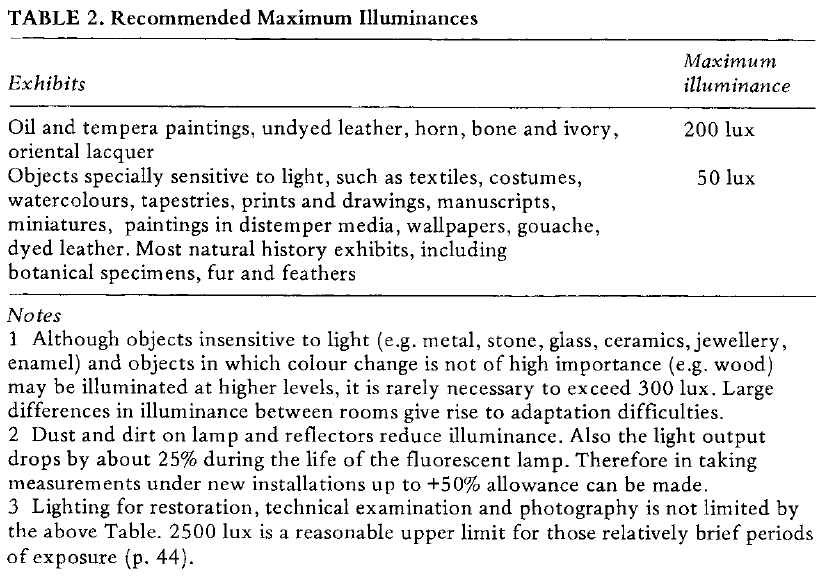
\includegraphics[max width=\textwidth]{figs/LitRev/Thomson.png}
\caption{Table 2 of \citet[p. 23]{thomson_museum_1986}, describing recommended maximum illuminances for 2 groups of objects.}
\label{fig:Thomson}
\end{figure}

Loe et al.'s work concludes with the recommendation that ``preferred artificial lighting conditions for viewing works of art are a painting illuminance approaching 200 lux provided from lamps with good colour rendering characteristics, e.g. a \gls{CIE}~R$_a$ index of \textgreater 85 and a large gamut area''. It is of particular interest to me that Thomson neglected to quote the final part of this recommendation regarding the specific \gls{CIE}~R$_a$ and note regards gamut area.

On the topic of colour rendering, Thomson goes into great depths to explain the topic and the means available for calculating various indices, spending a disproportionate amount of time (compared to what I understand was normal for the time) on the topic of Crawford's `band method' \citep{crawford_colour_1960,crawford_measurement_1959} for colour rendering index calculation amongst other things.

For the most part he neglects to make recommendations for specific target values, only making the rough and unsupported assertion in passing: 

\begin{itquote}{}
Recommendation for good colour rendering. \\
\gls{CIE}~R$_a$ about 90 or better, \\
R\textsubscript{w} (worst R) about 80 or better, \\
and Crawford Class A, B or C
\end{itquote}

No research is referenced to support this recommendation. The inclusion of $R$\textsubscript{w} (the lowest value of $R$\textsubscript{i}) is notable due to its lack of consideration in other documents. 

Still on the topic of colour rendering, of additional note is Thomson's general introduction to the subject, where he frames the conversation in a manner which presents colour rendering as a measure of the colour changes to which the human visual system is unable to adapt to, opposite changes induced by changes in colour temperature to which the human visual system is generally able to adapt easily to. Thomson also provides an accessible, and often quoted summary of the underpinnings of how the \gls{CIE} General Colour Rendering Index operates in principle:

\begin{itquote}{}
Adapt our eyes to the illuminant under test. \\
Look at a set of representative objects under it and accurately memorise their colours.\\
Adapt to the reference illuminant.\\
Look at the same objects under this second illuminant and compare the colours to the colours in our memory.
\end{itquote}

Thomson's comments on the selection of colour temperature are minimal, not referring to any specific \gls{CCT} in his summary of specifications [p. 268]. The only note dealing directly with the specification of colour temperature can be found on page 25, and refers only specifically to the conversation of what colour temperature to select for those environments which for conservation purposes need to be lit at particularly low illuminance levels.

\begin{itquote}{}
The `coolness' \dots of daylight when it has been reduced to 50 lux often gives the impression of gloom, especially when it is highly diffused. No one knows how deeply it has been built into our systems, but ever since our first ancestors sat around fires, and later used oil lamps and candles, the human race has been accustomed to `warm' light in the home after dark. As a result the warm 50 lux from tungsten lamps appears to be brighter, and certainly more cheerful, than 50 lux of diffused daylight. For the same reason warm rather than cool fluorescent lamps should be chosen for 50 lux situations.
\end{itquote}

It is assumed that the views expressed above are grown from empirical observation. They mirror the standpoint of other publications which refer to the work of \citet{kruithof_tubular_1941} and the derived `Kruithof curve' (see Section \ref{sec:CCTmus)}).

The bulk of pages 49-51 concern colour temperature, if one includes the associated discussion of chromatic adaptation and colour constancy, but there is no clear link as to how the author suggests that this theory should be considered in practical application, nor any concrete recommendations for target figures.

A final note in reference to this text goes to the discussion of whether or not to consider the type of lighting for which the artist intended an artwork to be displayed under, or that under which it was originally created. At the risk of quoting half the book I include one final passage which I think particularly pertinent to the area of research to be undertaken in this project, with which I shall conclude my discussion of this publication:

\begin{itquote}{}
I think one would be correct to suppose that artists have always assumed that their creations would be viewed in a variety of situations, not all lit ideally, and have designed their work accordingly. Even the Impressionists and others who made a point of completing their canvasses in the open air did not expect them to be so viewed. When De La Tour painted a candle-lit scene he painted it in such a way that the scene would look candle-lit under any reasonable lighting (for a contrary view see Weale [\citep{weale_truth_1973}]). 

But it could also be said that, however robust the work of art, it will look better in some lighting situations than in others, and so we should bend our efforts to finding the best possible situation. Within the limitations of the museum one cannot but agree, provided there is indeed a consensus of perceptive opinion on what is best, and provided that the damage caused by light is kept under control. 

There is certainly no mathematical treatment whereby we can equate the viewer's gain against the exhibit's loss. However there has been considerable research on the visual process as it is affected by the lighting, and Brommelle [\citep{brommelle_visual_1972}] has carefully related the experimental work to the museum problem.
\end{itquote}

\subsubsection{\gls{CIE} 157:2004 Control of Damage to Museum Objects by Optical Radiation}

This document is a \gls{CIE} technical report, prepared by \gls{CIE} Technical Committee 3-22 of Division 3 ``Interior Environment and Lighting Design''. 

To set the context for the discussion of this \gls{CIE} technical report, first a note to draw attention to the time period during which it was drawn up, since to the future reader there might be some ambiguity as to what the state of the art was at this point. Whilst it is now at the time of writing in 2016 common to find museums using LEDs to display their objects, this was not the case in 2004. It is noted within the text that LEDs are `are not of suitably high colour quality for museum use at present, but have future potential as very low UV power sources.' The increased use of LEDs does not invalidate the contents of this document, but it is worth considering that it was prepared with pretext to address any LED specific issues.

As previously mentioned, this document takes a different approach to the problem of limiting light induced damage in museums, focusing rather on the process of considering the optimal spectral power distributions as opposed to limiting the light levels wholesale. For example, the closest the document comes to making light level recommendations in the manner of `The Museum Environment' \citep{thomson_museum_1986} is in the tabulation of Mlx hour values for predicted noticeable fade. This approach leaves the decision of actual lighting levels to the museum professionals, with the question being `How long do I want this object to last before a noticeable fade has occurred?'

The document is in some ways an endorsement and extension of the approach taken by \citet{harrison_report_1953} (as discussed in Section \ref{sec:DamageIndex}), in which the concept of a damage function was introduced, this being ``an action spectrum that defines the relative spectral responsivity of a receiving material''. The authors of this document note that the work did not originally gain traction due to conservators' scepticism that a single function could represent the vast range of potential museum object (still an intractable problem). Interest was further lessened by the fact that the original work refers only to one very specific type of material - low grade paper. However, the authors of this document argue that the fundamental idea is sound; a damage function (so long as it is genuinely representative to an extent) could be a valuable tool in assessing the appropriateness of different light sources.

The authors then pull reference from further studies focused on a range of other materials, and find low grade paper is actually an outlier in terms of wavelength sensitivity, with many other materials able to be grouped together in type of dependency (if not like sensitivity). Following Cuttle's work \citep{cuttle_lighting_1988} to describe the pre-existing damage functions as simple mathematical relationships, comparison between the variety of newly created damage functions was possible.

Regarding colour temperature, the report states:

\begin{itquote}{}
While the variations of spectral responsivity for individual materials, particularly pigments, remains problematic, the overall tendency for responsivity to increase at shorter wavelengths is reasonably well defined. It has been shown that there is a general effect for the relative damage potential to increase as colour temperature increases [\citet{cuttle_lighting_1988}]
\end{itquote}

This falls short of offering recommendations for colour temperature choice, remaining impartially scientific. However, an included table, reproduced below, makes it clear that the lower the colour temperature, the lower the potential for damage (for a set SPD `type').

\begin{figure}[htbp]
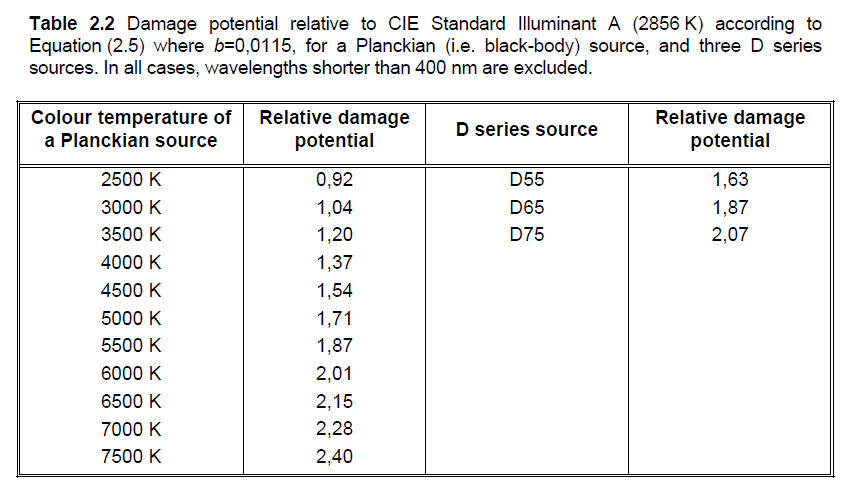
\includegraphics[max width=\textwidth]{figs/LitRev/CIE2004b.png}
\caption{Table 2.2 of \gls{CIE} 157:2004 \citep{cie_cie_2004}}
\label{fig:CIE2004b}
\end{figure}

This section concludes with the introduction of two related topics, again with significance for this project. The first regards the work of \citet{miller_evaluating_1993} in which the concept of \gls{REM} is introduced, the second is of the work by \citet{thornton_high_1975} in which he describes the technique of using `prime colour' light sources.

\gls{REM} in the current context refers to a process of illuminating an object preferentially with illumination of wavelengths which it is known to reflect. The premise of this is: absorbed radiation is visually unimportant, yet conversely the radiation most likely to damage an object. Thus an ideal situation would be to illuminate an object with radiation which it entirely reflects. The immediate limitations of this process are that this process would be object specific and potentially problematic for correct colour rendering. This procedure was suggested to be implemented using fibre optics and filter systems, it would likely be much more approachable with the advent of LED technologies which allow certain spectral flexibility.

A note in the text regards the potential for \gls{REM} to increase the saturation of colours relates that this `raises questions concerning the ethics of modifying the apparent colours of displayed objects.' 

\hl{Thornton/Prime}
\hl{(Colour rendering/critical viewing)}

In the final section of this document (written with the aim to `give recommendations for lighting in museums') very little advice is given in the form of specific figures to aim for, rather a decision appears to have been made that it was preferable to detail the areas that the authors considered worthy of attention, and to lay out the arguments for deliberation. For example, on the topic of \gls{CCT} choice reference is made to the previous discussion which details the deleterious potential of illumination at different colour temperatures, but it is clearly stated that `[w]here the viewing conditions call for moderate or high colour temperature lighting, conservation concerns should not override design objectives for the display.' This seems to be supported by the later statement that `[i]t is thoroughly bad policy to place an object on display, where it inevitably will suffer some damage, and to fail to present it adequately.' It is further noted that low colour temperatures may `judged unsatisfactory' when it is used in combination with natural illumination. 

With marked separation, the previously discussed work of \citet{loe_preferred_1982} is referred to, in the context of providing guidance on a lux value that is `generally sufficient to provide for adequate visibility'.

There is a noteworthy section on the meaningful distinction between illuminance and irradiance: `It needs to be recognised that illuminance is not a reliable alternative measure [for irradiance], as it represents the density of luminous flux, being radiant flux evaluated according to a typical human visual response, defined by the photopic spectral luminous efficiency function V($\lambda$). Not only does illuminance take no account of irradiance outside the visible spectrum, but also radiant flux within the visible spectrum is weighted according to its relative visual effect, which is not related to its damage effect.'

\subsubsection{CGI/Getty Guidelines for Selecting Solid-State Lighting for Museums}

This guidance document \citep{druzik_guidelines_2012}, produced by the Canadian Conservation Institute and The Getty Conservation Institute, provides guidance for museum professionals to select \gls{LED} lighting. As such, the guide includes an introduction to the technological theory of \glspl{LED}, advice on how to consider the requirements of museum lighting, and a practical guide to selecting lighting. It is the only document here considered which discusses solely LED technology.

Compared to the other documents considered here, there is also a focus on the longevity of systems, particularly in respect to potential for colour change, and advice on the type of information that should form a warranty agreement between supplier and end user.

A recurring piece of advice throughout the document is that a lighting specifier should always view lighting in person before making a significant order. The implicit, and sometimes explicit subtext here is twofold; firstly, that the specifications available for lighting are insufficient to describe the visual appearance of lighting, and secondly, that the quality of museum lighting (the ability of lighting to fulfil predetermined requirements) is visually assessable. An extension of this second point would be to consider the visual requirements in museums as being solely or principally defined by a general preference for appearance under lighting.

Following this notion, \gls{CIE}~R$_a$ is referred to as `imperfect' and `misunderstood', and it is suggested that it could be used as a `secondary consideration'. There are several different specific values of \gls{CIE}~R$_a$ recommended at different points within the document.

\begin{itquote}{}
It is generally agreed that a \gls{CRI} above 85 is suitable
\end{itquote}
\begin{itquote}{}
To illuminate areas with a more utilitarian [function] such as machinery, many science exhibits, food services, hallways, educational activities, etc. settle on a color rendering index (\gls{CRI}) above 80. When color matching may be more an attentive activity such as viewing art, ethnography, some natural history collections exhibits, etc. select \glspl{LED} with a \gls{CRI} above 90. However, because \gls{CRI} is an imperfect metric, \gls{CRI} should be considered a target, not a firm criterion.
\end{itquote}
\begin{itquote}{}
There is no international museum standard on what is or is not an ``acceptable'' \gls{CRI}, but the Canadian Conservation Institute (CCI) recommends a minimum of 85. Many museums specify greater than 90.
\end{itquote}

As is perhaps apparent in the quotes above, this document has the feel of friendly advice rather than an official guidance document. As such, it has particular value for this project as a perhaps more revealing account of the advice which actually circulates in the field. For example, one piece of advice which I haven't seen anywhere else in official literature, but which as I understand it is relatively common in general parlance is that provided during the overview on page 23: `Check color rendering on your own skin'. This advice is incongruous with the museum lighting advice which prioritises objectivity and impartiality, as this implicitly suggests looking for a `pleasing' appearance.

The document makes subtle references to the \gls{CQS} \citep{ohno_rationale_2010,baier_is_2012,davis_toward_2005,davis_color_2010} and \gls{GAI} \citep{rea_color_2008}; saying that in response to limitations with \gls{CIE}~R$_a$ `at least two other color metrics have been proposed recently', followed by references which relate to the aforementioned respectively. The document also makes two references specifically to \gls{CIE}~R$_9$ values, firstly as part of the information on the ENERGY STAR program (where it is quoted alongside other lamp specifications) and once in the Appendix (where visual demonstrations of induced colour shifts are provided for the \gls{CQS} and \gls{CIE} test colour samples. Interestingly, a scale for \gls{CIE}~R$_9$ is described, where: `\gls{CIE}~R$_9$ = 0-49 means it renders red hues well. When R9 is 50-74 it is very good. R9 above 75 is considered excellent.' As with many items in this document, no reference as to the source of this information is provided. 

Regards the question of CCT within museum lighting, the guidance offers a Kruithof-ian approach, though without naming it as such, recommending warmer light for lower light levels and colder light for higher light levels. 

\begin{itquote}{}
With low light levels, as in museums, viewers tend to prefer warmer light similar to that of incandescent lamps, e.g. the 2800K of standard incandescent lamps, or the slightly higher 3000K of quartz halogen incandescent lamps. As illumination increases to several thousand lux, preference is for cooler light, 5000K or higher.
\end{itquote}

It is noted than an exception might be made in the situation where artificial lighting is employed to augment natural illumination. This said, elsewhere in the same document the reader is advised to `avoid higher color temperatures for light sensitive materials as these LEDs may have an unacceptably large peak in the ``blue region'' of the spectrum.'

Also poorly referenced is the discussion of the 50 lux recommendation. Research is mentioned but not directly quoted. It is assumed that the research described as `in the 1980s' is the previously discussed research of \citep{loe_preferred_1982}.

The final area of note within this report is that which considers the methods applicable to assessing museum lighting in situ. A survey completed at the Field Museum \citep{myer_demonstration_2010} is quoted in detail, the survey having been completed by museum staff and lighting practitioners as part of a GATEWAY program demonstration at the museum. This survey includes such questions as `The lighting product shows \underline{\hspace{2cm}} of the subject colors accurately' and was completed for a halogen system and an LED system in the same space.

\subsubsection{SLL LG8: Lighting for museums and art galleries}

\citet{cibse_lighting_2015}

% To be written up
% -	Recent doc 2015
% -	Benefits from Practical examples
% -	Lots of big/familiar names
% -	Limited references, no in line sources

% -	Pg 3 CCT warmer light standout?
% -	Pg 4 CRI 90 very good, <80 not suitable
% -	5 colour of backgrounds
% -	9/12 combining daylight and cct
% -	24 `purely advisory' reflect current practice
% -	25 `access has two components, visibility and duration of exposure to light'
% -	27 basing on `good eyesight' might be `discriminatory'
% -	28 distorting intention of artist
% -	33 V&A JNC 50years?
% -	43 trade off
% -	46 blue peak ongoing research
% -	47 essential to conduct side-by-side trials
% -	67 good colour quality = poor efficacy?
% -	Many specific object types

\subsubsection{IES RP-30-96 Museum and Art Gallery Lighting: A Recommended Practice}

\citet{ies_ies_1996}

% -	1996, as of 2016 being updated
% -	Guide for lighting designers

% -	1 `human achievement'
% -	1 Different priorities for different people (kesner)
% -	1 Three rules
% -	2 `Color should not change the look of an artifact' ``overriding – original appearance''
% -	3 CRI ``true color'' >80
% -	3 CCT Determine whether the display takes on a warm or cool appearance
% -	12 30lux required for color
% -	12 avoid bold surrounding colours
% -	13 `killing the patient'
% -	15 lux = exposure(?)
% -	31 Brief history of daylight in galleries
% -	31 adaptation



















\subsection{CCT in museums}
\label{sec:CCTmus}

\Gls{CCT} is often described as an important variable in museum lighting, but definite recommendations, in the rare cases that they are given, are generally based on nostalgia for the appearance of tungsten lighting, questionable research on human preference \citep{kruithof_tubular_1941,fotios_revised_2017} or very rough rules that predict that damage potential will be decreased if \gls{CCT} is minimised \citep{cie_cie_2004}. Whilst some research appears to have found optimal \glspl{CCT} for viewing artwork \citep{nascimento_best_2014,pinto_correlated_2008,scuello_museum_2004,scuello_museum_2004-1, liu_cultural_2013,vidovszky-nemeth_introductory_2016,feltrin_impact_2019} results often have large inter-observer variability, context dependency and it is not uncommon for the headline findings of separate studies to be in contradiction. 

Specifications often refer implicitly or explicitly to the findings of \citet{kruithof_tubular_1941}, who found that at lower levels of illumination, lower \glspl{CCT} were preferred, and that at higher levels of illumination higher \glspl{CCT} were preferred (see Figure \ref{fig:Kruithof}). Whilst this general trend seems to have anecdotal support, it is possible that there may be lighting-technology-based confounds, and recently researchers \citep{vienot_kruithofs_2009} (including a meta-study of multiple other examinations \citep{fotios_revised_2017}) found there to be no substantive support for Kruithof's findings.

% Kruithof is referred to a lot but needs proper discussion somewhere. %DG: I think I do that already above (?)

\begin{figure}[htbp]
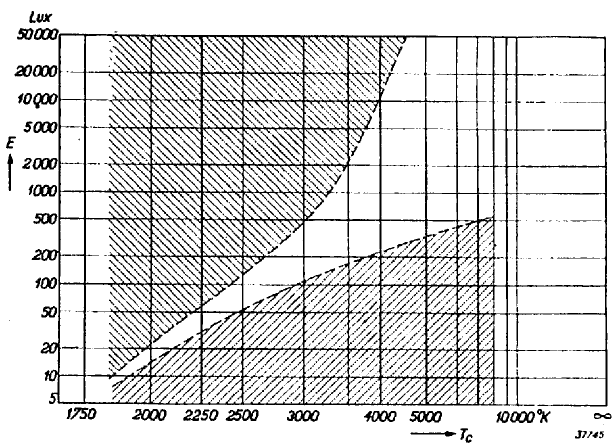
\includegraphics[max width=\textwidth]{figs/LitRev/Kruithof.png}
\caption{The `Kruithof curve' reproduced from \citet{kruithof_tubular_1941}, showing colour constancy against illuminance, and highlighting an area that is considered ``pleasing'' (central white area).}
\label{fig:Kruithof}
\end{figure}

The damage justification seems more substantive; following the application of damage factors as discussed in Section \ref{sec:DamageIndex} the \gls{CIE} published a report showing the varying the \gls{CCT} of museum lighting could have a clear impact on the potential damage undergone by museum objects \citep{cie_cie_2004}. 

\begin{figure}[hbtp]
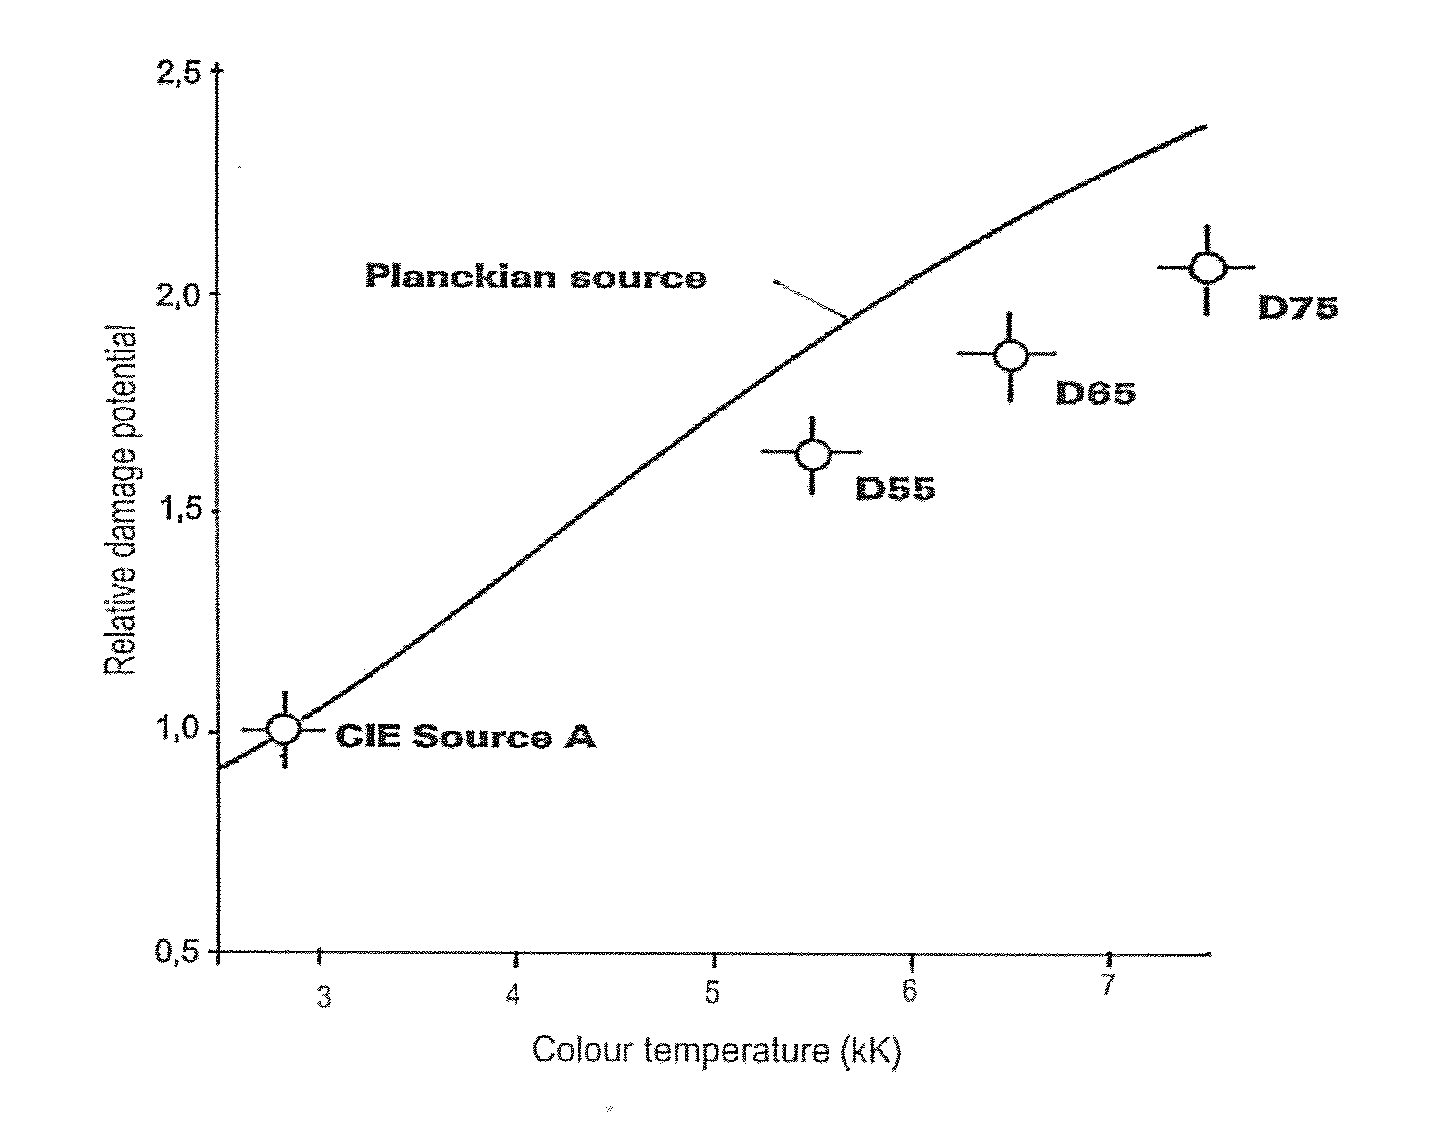
\includegraphics[max width=\textwidth]{figs/LitRev/CIE2004.png} 
\caption{Figure reproduced from \gls{CIE} 157:2004 \citep[p.16]{cie_cie_2004}, showing the relationship between \gls{CCT} and relative damage potential for black body radiator illuminants, \gls{CIE} source A and three \gls{CIE} D-series illuminants.}
\label{fig:CIE2004}
\end{figure}

This line of reasoning relies heavily upon the applicability of damage functions to the specific materials in question. As discussed previously (Section \ref{sec:DamageIndex}) it seems that whilst the generalised damage functions account for some of the individual material damage functions, they do not fully do so. However, tentatively, they do seem to be a relatively good fit for the shared characteristics of different damage functions (at least far more so than V($\lambda$)), and so it seems reasonable to use them where no other broad approximation for a large set of objects exists.

To verify the findings of the \gls{CIE}, extend their findings to \glspl{LED}, and provide code for others to do similar research or even test their own lights/materials, a set of MATLAB functions\footnote{\url{https://github.com/da5nsy/DamageIndex/blob/c7851e27ca1b0915013d8723db04704b49b4085e/CalcDI.m}} have been written (by the author) which calculate \gls{DI} values for arbitrary illuminants. This code has been used to produce Figure \ref{fig:CCTvsDI}, which shows the \glspl{CCT} and \glspl{DI} of the 401 \glspl{SPD} of \citet{houser_review_2013}. A $b$ value of 0.0115 corresponding to `oil paints on canvas' and `water colours on rag paper' (see Table \ref{tab:b}) was used. It can be seen that there is a clear correlation between \gls{CCT} and \gls{DI} with higher \glspl{CCT} being predicted to be relatively more damaging. If a damage function with a lower $b$ value (such as for `low-grade paper' or `textiles') had been used, the relationship between \gls{CCT} and \gls{DI} would be steeper.

%\afterpage{\clearpage}
%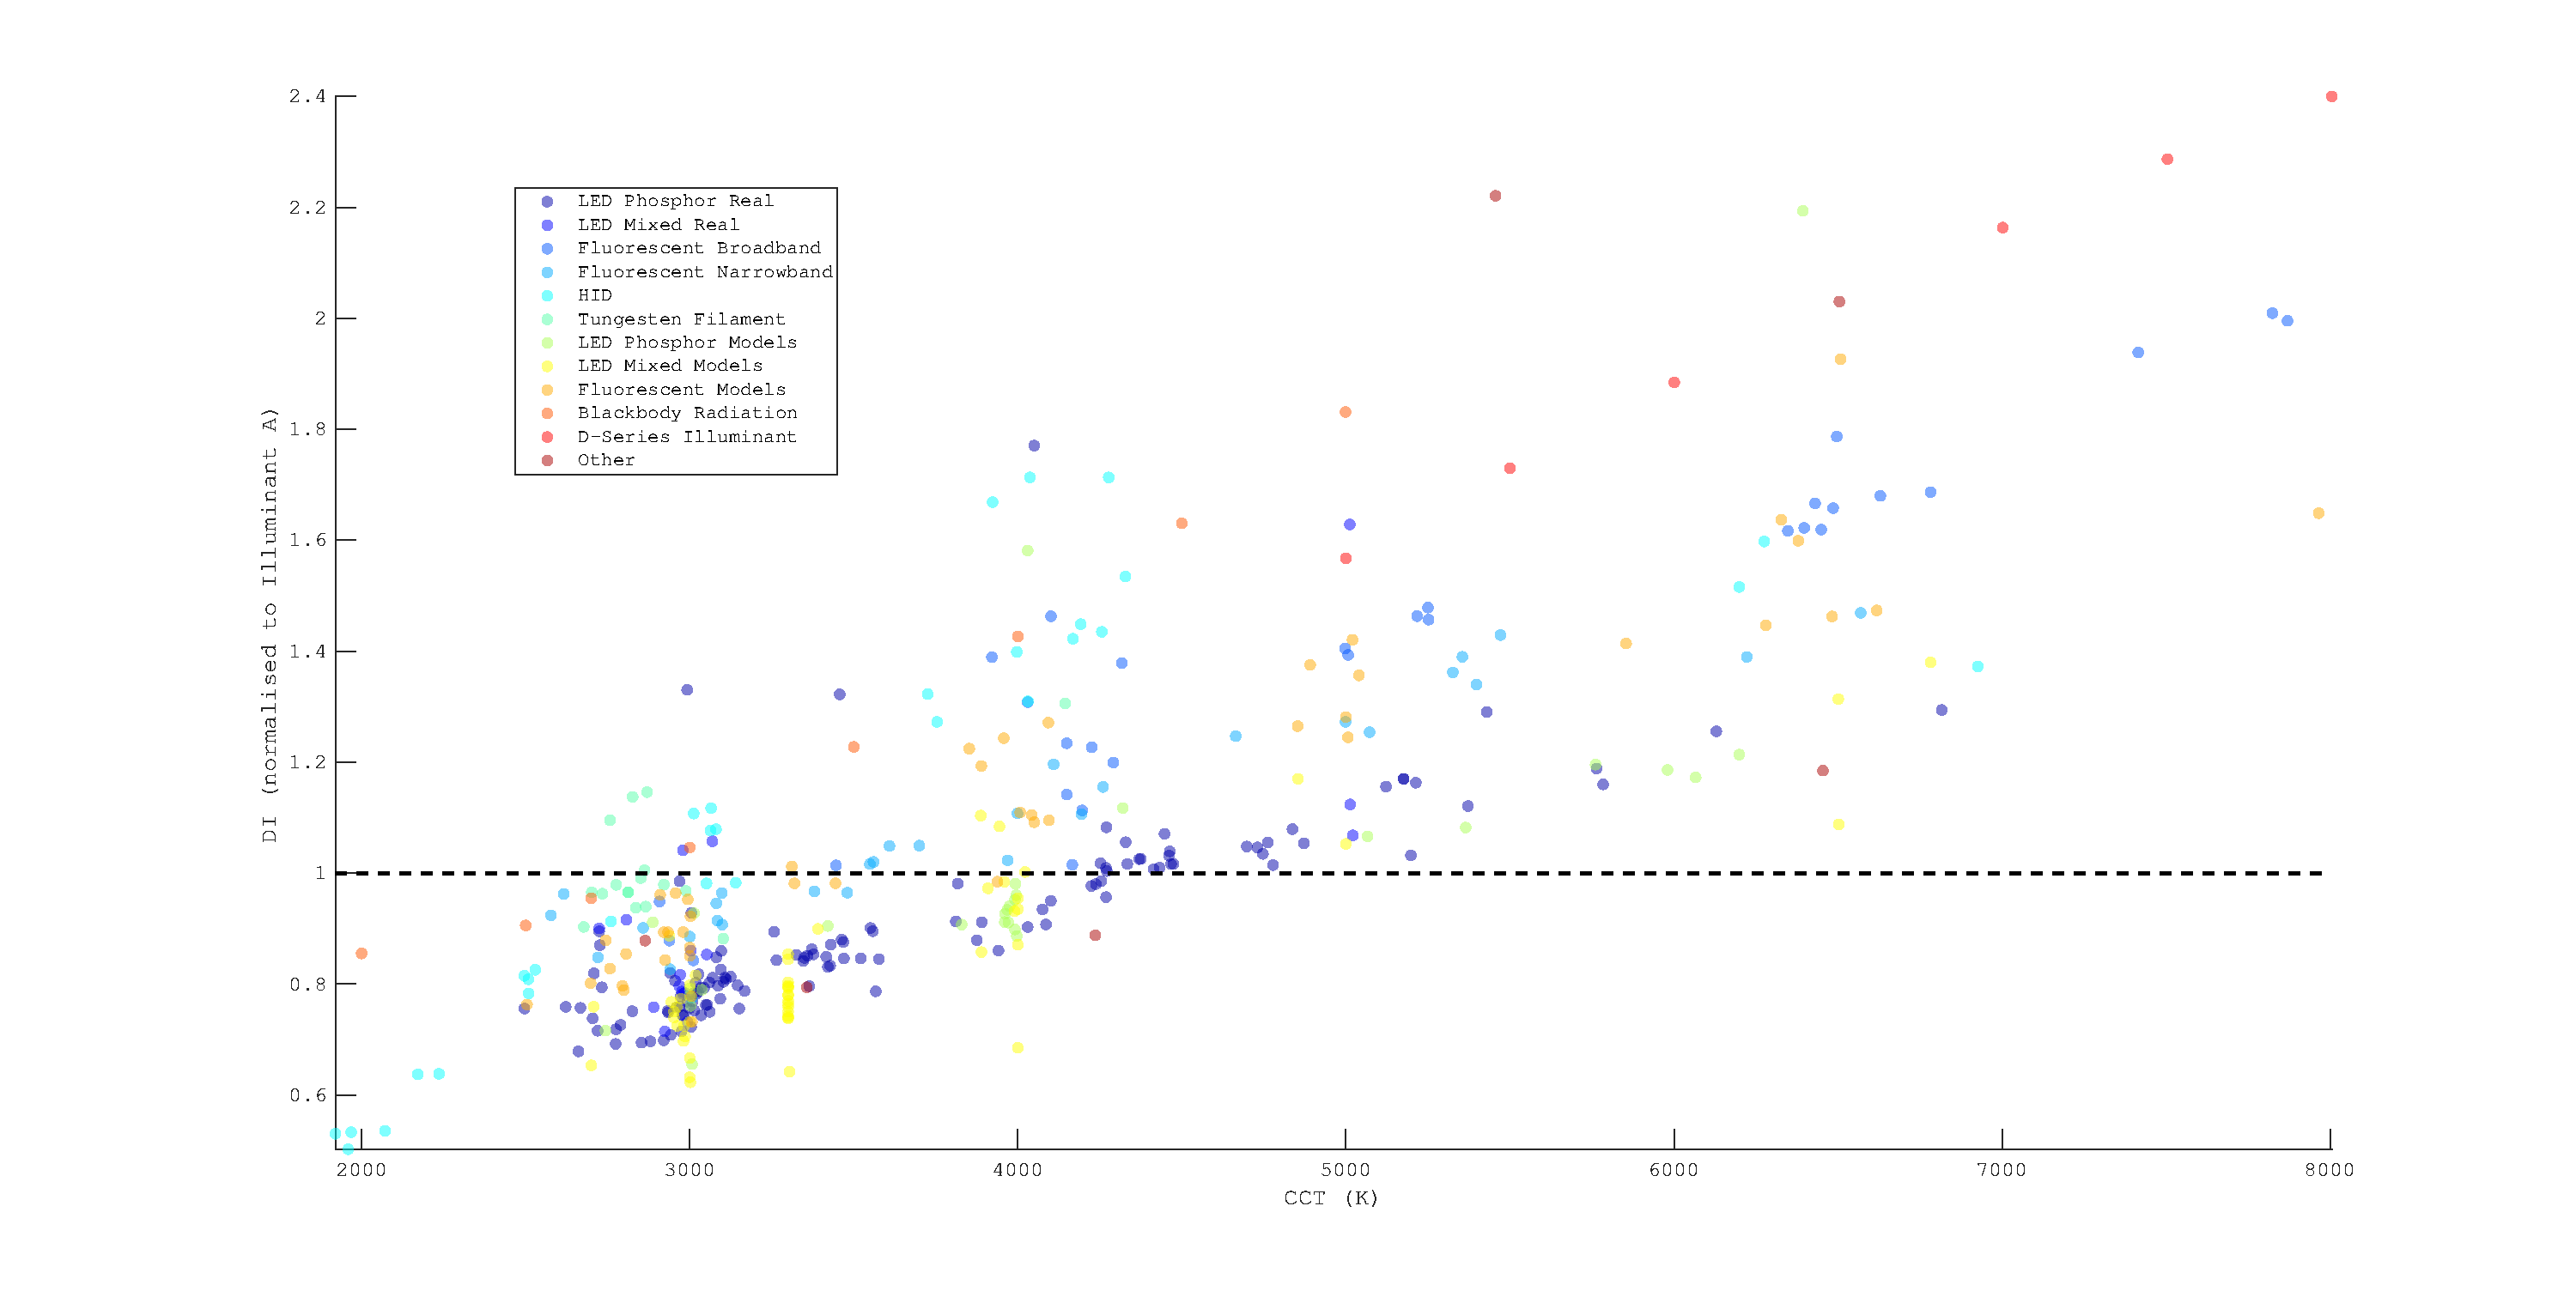
\includepdf[pages=-,rotate=90, offset=75 -75]{figs/LitRev/CCTvsDI.pdf}
% \begin{figure}[t]
%     \caption{The \glspl{CCT} and \glspl{DI} of the \glspl{SPD} used by \citet{houser_review_2013} [provided via personal communication, but now partially available via \gls{PTB} as `spd\_houser'].}
%     \label{fig:CCTvsDI}
% \end{figure} 

\begin{fullpagefigure}
\figpdf[pages=-,rotate=90, offset=-85 -85]{figs/LitRev/CCTvsDI.pdf}
\figpageside{}
\caption{The \glspl{CCT} and \glspl{DI} of the \glspl{SPD} used by \citet{houser_review_2013} [provided via personal communication, but now partially (without category information) available via \gls{PTB} as `spd\_houser'].}
\label{fig:CCTvsDI}
\end{fullpagefigure}

The results of these computations show a clear relationship between \gls{CCT} and \gls{DI}. Considering that this is not currently taken advantage of in museum lighting, it seems as though there is a great potential for reducing damage whilst maintaining visitor visual satisfaction.

%\clearpage
% This is combo with the figpageside thing above currently isn't quite working

%%%% !!!!!!!!!! Check this works before printing

\cleardoublepage %works but seems a bit heavy handed.

\subsection{Colour Rendering Indices in Museums}

%Are fidelity indices suitable for museum use? 
The first chapter of Cuttle's book `Light for Art's Sake: Lighting for Artworks and Museum Displays' \citep{cuttle_light_2007} is titled `A philosophy for the presentation of art'. The choice of title here is apt but may surprise some readers, sounding more whimsical than might be expected of a serious subject attended by scientists and engineers. The reason it is so apt is because lighting is unavoidably a creative intervention\footnote{Credit for this phrase to Katherine Curran} which is to say that there is no lighting which is truly impartial, and no lighting which is truly `correct' in the sense of being unequivocally superior to another. All lighting decisions require choices to be made, and whilst these choices can be wrapped up to appear as an optimisation problem where proximity to a particular solution is the goal, the problem always rests on the bedrock of a philosophy based decision.

In the above mentioned chapter Cuttle lays out a total of seven distinct philosophical propositions, which he poses for consideration as approaches to museum lighting, some contradictory and some with the potential to overlap:

\begin{enumerate}
\item To make the artwork appear as it would have appeared to the artist at the time of its creation
\item To ensure that no damage due to light exposure will occur
\item To achieve the best possible appearance of the artwork
\item To provide optimum conditions for viewing art
\item To impart a sense of having seen `the real thing'
\item To assist viewers to understand the displayed objects and their reason for being there
\item For the lighting designer to establish a distinct and recognisable style
\end{enumerate}

These propositions refer to museum lighting holistically, considering all aspects of museum lighting, but can be readily focused on the problem of colour appearance specifically. Before we narrow our gaze however, it is worth briefly considering a wide view of lighting attributes which may aid in the realisation of `good quality' museum lighting. Consider Rosenfeld's list of the five `controllable qualities' in museum lighting; `intensity, movement [temporal artefacts], angle [modelling, avoiding glare and reflections], distribution [ambient lighting vs. spot lighting], color' \citep{rosenfeld_agony_2013}.

Whilst Cuttle's propositions make for interesting discussions and enjoyable extended pondering, they are of limited assistance in the practical task of actually specifying lighting. Thankfully, a range of tools exist for the examination of the colour rendering properties of a light source, in the form of indices which aim to numerically describe an illumination's effect on colour appearance of the objects of which it is tasked with illuminating.

Traditionally, colour rendering indices aim to offer a standardised method for calculating the colour differences induced by the substitution of a reference illuminant with a specific test source, and for comparing the relative merit of different test light sources on their ability to induce minimum change. In modern parlance this type of index should be referred to as a colour fidelity index, that is - one which is conceptually concerned with colorimetric reproduction. The term `colour rendering' has come to encompass much more than just fidelity.

Diametrically opposed in some ways to fidelity are the indices which aim to quantify `preference'. In the simplest case, a preference index will aim to provide a value that is predictive of how an observer would rate a light source against other light sources. 

Within and between these two groups there exist a range of different indices with subtly different aims and mechanisms for achieving these aims. For thorough overviews see \citet{guo_review_2004} and \citet{houser_review_2013}.

In practice, both of these philosophical approaches are mandated in current lighting guidance. For the most part, advice for lighting specification on the subject of colour rendering can be simplified to read `use lamps of above \gls{CRI} 80 (referring tacitly to \gls{CIE}~R$_a$) but always test them visually before you buy in bulk'. Whilst this may at first seem like sensible advice, upon further inspection it actually represents a serious contradiction, unless considered with heavy caveats. The problem rests in the fact that \gls{CIE}~R$_a$ is a fidelity index, whereas any visual inspection is likely to be performed by observing the appearance of an object under the test illumination without a reference. Fidelity aims to describe accuracy of reproduction, but this is a quality which is arguably not testable by visual inspection. This contradiction seems to perpetuate unnoticed in museum practice, with lighting specifiers often abstractly declaring to target a faithful/accurate/honest/impartial representation of objects, but practically choosing light sources based on visual inspection where preference is the only criteria. There is of course a range of approaches, ranging from pure reliance on indices to almost entire reliance on visual testing.

In conclusion, no one metric exists that would satisfy the divergent aims and philosophies of museum lighting. Several distinct types of colour rendering index exist, but the existing range fall into the broad categories of `fidelity' or `preference', with the latter being particularly poorly definable due to its variability in different environments, with different user functional requirements and different intrinsic preferences between different observers. Progress could be made by breaking these broad categories into smaller more manageable specific objectives.

%weale_truth_1973

%vienot birds
% vienot_leds_2011

%bespoke colour rendering indices, sistine chapel
% schanda_new_2014

%correcting for hunt effect
% wei_consideration_2018



%%%% BONUS AREA %%%%%%%%%%


%\subsection{LEDs in museums}

%%%%%%%%%%%%%%%

%Theoretically, there exists a division between recommendations which deal with visual appearance and those which deal with physical degradation; the first group supported by the science of human vision, and the second supported by material sciences and chemistry. Whilst it is important to be aware of this distinction, it is normally not possible to consider them entirely separately in practice, as many variables will affect both.

%%%%%%%%%%%


%Extending the question of visibility is the subject of appearance. It is a general expectation that museums represent objects in a truthful and impartial manner, and it seems sensible that decisions concerning the appearance of items in museums should be made with this in mind. Alongside this, many museums treasure items where part of their value is aesthetic2, and it follows therefore that a technique which aids in the beautification of an object might be of interest, and this might be particularly of interest if the object is known to have deteriorated since the time of production.

%%%%%%%%%%%

% \subsection{Lighting at The British Museum}

% Lighting at the British Museum has developed in a somewhat organic manner, from the early days of the museum before the introduction of artificial lighting. This leaves the museum with more than sufficient daylight in most spaces during daylight hours, where the increased modern knowledge regarding the deleterious effect of lighting now means that conservators must find ways in which to limit this natural resource so that objects are not unduly exposed. 

% The gallery lighting is replaced when a gallery is refurbished, and the latest technology is installed when a new gallery is created, where viable in terms of suitability and considering financial limitations. Other than this, lighting technologies tend to not be updated other than to replace individual lamps. This coupled with the grand scope of the museum, which means that it is rare for multiple galleries to be refurbished simultaneously, has led to a vast array of lighting designs and technologies. It in fact appears to represent a rather special example of `museum lighting through the ages', with daylight, tungsten, fluorescent and metal halide lamps all seemingly represented, as well as various illumination geometries reminiscent of the times of their fitting. It should be noted that these assertions are made following empirical observation with spectrophotometers and not from conversations with museum staff, see section 3.3 Collection of \gls{SPD} Data at British Museum.

% There also seems to be a great range of lighting quality within the British Museum, with some spaces feeling bright and others comparatively gloomy. There is a range of colour temperatures and chromaticities of light at the museum, as shown in Figure 1.

% Multiple methods are currently employed to limit the exposure of objects in the museum. \Gls{UV} absorbing film or glazing which incorporates \gls{UV} reduction is used throughout the museum and in certain galleries there are automatic blinds which limit the intrusion of direct sunlight at specific times of the day and year. For particularly sensitive objects, rooms are lit artificially at very low levels, and some objects are selectively lit in order to further limit their accumulative exposure.

% 

\section{Mathematical Methods}

A small number of mathematical methods which may not be familiar to the reader are used within this thesis. They are outlined below.

\subsection{K-means clustering}
\subsection{Principal Component Analysis}


